\chapter{Planung und Konzeption}
\section{Funktionale Anforderungen}
Die Kursräume stellen das Kernkonzept dar; sie können erstellt, gelöscht, abonniert, deabonniert und Nachrichten in sie eingestellt werden.
Ein Benutzer muss sich beim Start der Applikation mit seinem eindeutigem Nutzernamen und dem zugehörigem Passwort authentifizieren.
Die Anwender sind in drei Kategorien eingeteilt: Student, Professor und Administrator.
Je nach Rolle des Benutzers wird die jeweilige Oberfläche angezeigt.
Im Folgenden wird das Kursraumkonzept und die jeweiligen Rollen genau beschrieben.

\subsection{Kursraumkonzept}
Ein Kursraum ist im Normalfall einem Kurs, der aus einem Professor und einer beliebigen Anzahl an Studenten besteht, zugeordnet.
Er wird vom Dozenten erstellt und die Studenten können ihn anschließend abonnieren.
Stellt der Kursraumersteller nun eine Nachricht ein, wird diese an jeden Abonnenten weitergeleitet.
Ein Dozent kann eine beliebige Anzahl an Kursräumen erstellen und von ihm erstellte auch wieder löschen.
Ein Student kann mehrere Kursräume abonnieren und wieder deabonnieren.
Abbildung \ref{pic:kursraumkonzept} visualisiert das eben Erläuterte.
\begin{figure}[H]
	\begin{center}
	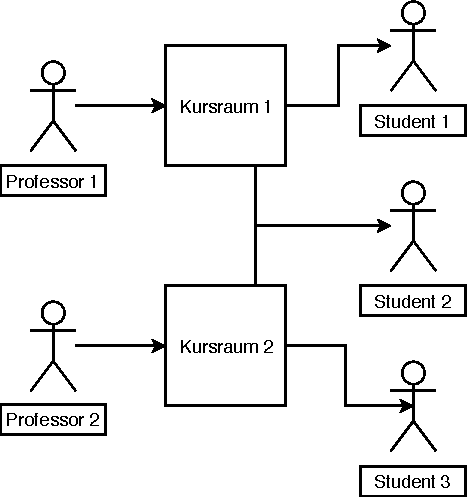
\includegraphics[scale=1]{Resources/KursraumKonzept}
	\caption{Visualisierung des Kursraumkonzeptes}
	\label{pic:kursraumkonzept}
	\end{center}
\end{figure}
\newpage
\subsection{Rollen}
In den folgenden Abschnitten werden die Benutzerrollen und die speziellen Anwendungsfälle genau definiert.
Alle Benutzer haben gemein, dass sie sich vor dem Benutzen der Applikation mit Passwort und Benutzernamen authentifizieren müssen.
Die jeweiligen Rollen sind in der Datenbank hinterlegt.
\subsubsection{Dozent}
Ein Dozent kann Kursräume erstellen und diese wieder löschen.
In einem von ihm erstelltem Raum kann er Nachrichten einstellen, die an alle Abonnenten dieses Raumes weitergeleitet werden. 
\begin{figure}[H]
	\begin{center}
	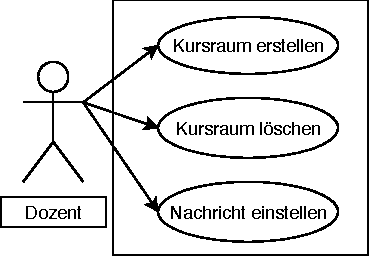
\includegraphics[scale=1]{Resources/UseCaseDozent}
	\caption{Berechtigungen für Benutzer in der Rolle \enquote{Dozent}}
	\label{pic:UseCaseDozent}
	\end{center}
\end{figure}
\subsubsection{Student}
Ein Student ist dazu berechtigt Kursräume zu abonnieren und zu deabonnieren.
Er empfängt alle Nachrichten, die in von ihm abonnierten Kursräumen eingestellt wurden.
Es können nur Kursräume deabonniert werden, die zuvor abonniert wurden.
\begin{figure}[H]
	\begin{center}
	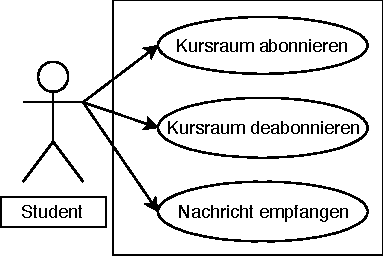
\includegraphics[scale=1]{Resources/UseCaseStudent}
	\caption{Berechtigungen für Benutzer in der Rolle \enquote{Student}}
	\label{pic:UseCaseStudent}
	\end{center}
\end{figure}
%\subsubsection{Administrator}
%Administratoren erhalten eine Übersicht über alle Benutzer und die ihnen zugeordneten Rollen.
%Er ist dazu berechtigt einen Studenten in einen Dozenten umzuwandeln und umgekehrt.
%Die Rolle \enquote{Administrator} kann nicht über die Android-Applikation vergeben werden.
%\begin{figure}[H]
%	\begin{center}
%	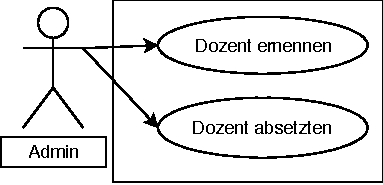
\includegraphics[scale=1]{Resources/UseCaseAdmin}
%	\caption{Berechtigungen für Benutzer in der Rolle \enquote{Administrator}}
%	\label{pic:UseCaseAdmin}
%	\end{center}
%\end{figure}

\newpage
\subsection{Anwendungsfälle für Studenten}
\subsubsection{Kursraum abonnieren}
\begin{center}
  \begin{table}[H]
    \begin{tabular}{| a | p{10cm} |}
      \hline
      Use-Case & Ich möchte über eine einfache Gesamtansicht alle verfügbaren Kursräume betrachten und abonnieren können, sodass diese meinem Account hinzugefügt werden. \\
      \hline
      MuSCoW & MUST
    \end{tabular}
  \caption{Anwendungsfall Abonnieren}
  \label{use-case-abbonieren}
  \end{table}
\end{center}

\subsubsection{Kursraum de-abonnieren}
\begin{center}
  \begin{table}[H]
    \begin{tabular}{| a | p{10cm} |}
      \hline
      Use-Case & Ich möchte in einer einfachen Gesamtansicht alle Kursräume betrachten, die ich abonniert habe und sie gegebenenfalls de-abonnieren. \\
      \hline
      MuSCoW & MUST
    \end{tabular}
  \caption{Anwendungsfall De-Abonnieren}
  \label{use-case-deabonnieren}
  \end{table}
\end{center}

\subsubsection{Nachrichten ansehen}
\begin{center}
  \begin{table}[H]
    \begin{tabular}{| a | p{10cm} |}
      \hline
      Use-Case & Ich möchte alle Nachrichten aller Kursräume, die ich abonniert habe betrachten. Diese sollen nach Einstellzeitpunkt sortiert sein. \\
      \hline
      MuSCoW & MUST
    \end{tabular}
  \caption{Anwendungsfall Nachrichten ansehen}
  \label{use-case-view-messages}
  \end{table}
\end{center}

\subsection{Anwendungsfälle für Dozenten}
\subsubsection{Meine Kursräume anzeigen}
\begin{center}
  \begin{table}[H]
    \begin{tabular}{| a | p{10cm} |}
      \hline
      Use-Case & Ich möchte in einer Übersicht alle Kursräume sehen, die ich erstellt habe. \\
      \hline
      MuSCoW & MUST
    \end{tabular}
  \caption{Anwendungsfall erstellte Kursräume anzeigen}
  \label{use-case-show-classrooms}
  \end{table}
\end{center}

\subsubsection{Kursraumübersicht anzeigen}
\begin{center}
  \begin{table}[H]
    \begin{tabular}{| a | p{10cm} |}
      \hline
      Use-Case & Ich in einer Kursraumansicht alle Nachrichten sehen, die ich in diesen Raum eingestellt habe. \\
      \hline
      MuSCoW & MUST
    \end{tabular}
  \caption{Anwendungsfall Kursraumübersicht anzeigen}
  \label{use-case-show-classroom}
  \end{table}
\end{center}

\subsubsection{Kursraum erstellen}
\begin{center}
  \begin{table}[H]
    \begin{tabular}{| a | p{10cm} |}
      \hline
      Use-Case & Ich möchte einen Kursraum erstellen, den meine Studenten abonnieren können. \\
      \hline
      MuSCoW & MUST
    \end{tabular}
  \caption{Anwendungsfall Kursraum erstellen}
  \label{use-case-create-classroom}
  \end{table}
\end{center}

\subsubsection{Kursraum löschen}
\begin{center}
  \begin{table}[H]
    \begin{tabular}{| a | p{10cm} |}
      \hline
      Use-Case & Ich möchte einen erstellten Kursraum löschen. \\
      \hline
      MuSCoW & MUST
    \end{tabular}
  \caption{Anwendungsfall Kursraum löschen}
  \label{use-case-delete-classroom}
  \end{table}
\end{center}

\subsubsection{Nachricht in Kursraum einstellen}
\begin{center}
  \begin{table}[H]
    \begin{tabular}{| a | p{10cm} |}
      \hline
      Use-Case & Ich möchte eine neue Nachricht in einen Kursaum, den ich erstellt habe, einstellen. \\
      \hline
      MuSCoW & MUST
    \end{tabular}
  \caption{Anwendungsfall Nachricht in Kursraum einstellen}
  \label{use-case-post-message}
  \end{table}
\end{center}

\subsubsection{Nachricht aus Kursraum entfernen}
\begin{center}
  \begin{table}[H]
    \begin{tabular}{| a | p{10cm} |}
      \hline
      Use-Case & Ich möchte eine Nachricht aus einen Kursaum, den ich erstellt habe, entfernen. \\
      \hline
      MuSCoW & MUST
    \end{tabular}
  \caption{Anwendungsfall Nachricht aus Kursraum löschen}
  \label{use-case-delete-message}
  \end{table}
\end{center}

\subsection{Weitere Anforderungen}
\subsubsection{Filtern}
\begin{center}
  \begin{table}[H]
    \begin{tabular}{| a | p{10cm} |}
      \hline
      Requirement & In einer Übersichtsansicht (Kursräume, Nachrichten etc.) sollen die Dargestellten Daten gefiltert werden können. \\
      \hline
      MuSCoW & SHOULD
    \end{tabular}
  \caption{Anforderung Filtern}
  \label{requirement-filtering}
  \end{table}
\end{center}

\subsubsection{Aktualisieren}
\begin{center}
  \begin{table}[H]
    \begin{tabular}{| a | p{10cm} |}
      \hline
      Requirement & In einer Übersichtsansicht (Kursräume, Nachrichten etc.) sollen die dargestellten Daten manuell aktualisiert werden könne. \\
      \hline
      MuSCoW & SHOULD
    \end{tabular}
  \caption{Anforderung Aktualisierung}
  \label{requirement-refresh}
  \end{table}
\end{center}

\section{Oberflächen}
Im Nachfolgendem werden die Benutzeroberflächen der Applikation, die enthaltenen Bedienelemente und deren jeweilige Funktion beschrieben.
\subsection{Authentifizierung}
Zu Beginn einer Sitzung muss sich jeder Anwender -- unabhängig von seiner Rolle -- mit seiner E-Mailadresse und dem zugehörigem Passwort anmelden. 
Es sind nur E-Mailadressen der Hochschule Landshut zulässig.
Die Bedienungsoberfläche für den ersten Benutzungsschritt wird in Abbildung \ref{pic:ActivityLogin} dargestellt.
Im Feld \enquote{Email} wird die Mailadresssee des Anwenders und analog dazu im Feld \enquote{Passwort} das Passwort eingetragen.
Durch Klick auf den Knopf \enquote{Sign In} startet ein Authentifizierungsversuch.
Zunächst überprüft die Applikation die syntaktische Korrektheit der Mailadresse und informiert gegebenenfalls über ungültige Eingaben.
Im Falle einer validen Eingabe werden die Anmeldedaten an den Server geleitet und mit der Datenbank abgeglichen.
Existiert ein Benutzer mit den jeweiligen Daten, so wird die zugeordnete Rolle übermittelt.
Abhängig von der Antwort des Servers öffnet sich dann die Oberfläche \enquote{\nameref{section:DozentenOberflache}} oder 
\enquote{\nameref{section:StudentenOberflache}}.

\begin{figure}[H]
	\begin{center}
	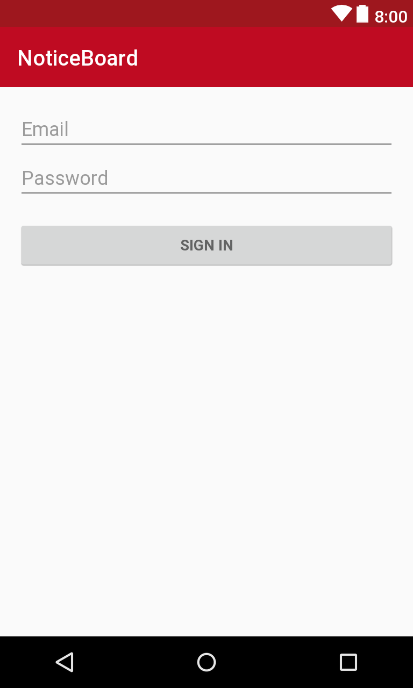
\includegraphics[scale=0.15]{Resources/ActivityLogin}
	\caption{Oberfläche für das Anmelden in der Applikation}
	\label{pic:ActivityLogin}
	\end{center}
\end{figure}

\subsection{Oberfläche für Dozenten}\label{section:DozentenOberflache}
Hat sich ein Nutzer der Rolle \enquote{Dozent} erfolgreich angemeldet, so erscheint die Oberfläche \enquote{MyClassrooms}.
Hier werden alle Klassenräume angezeigt, die er verwaltet.
Der Dozent hat nun die Möglichkeit entweder über den Button mit dem Löschen-Symbol Klassenräume und alle enthaltenen Nachrichten zu löschen (siehe Abbildung \ref{pic:LecturerDeleteClassroom}) oder über den Button unten Rechts einen neuen Klassenraum zu erstellen (siehe Abbildung \ref{pic:LecturerCreateClassroom}). 

\begin{figure}[H]
	\begin{center}
	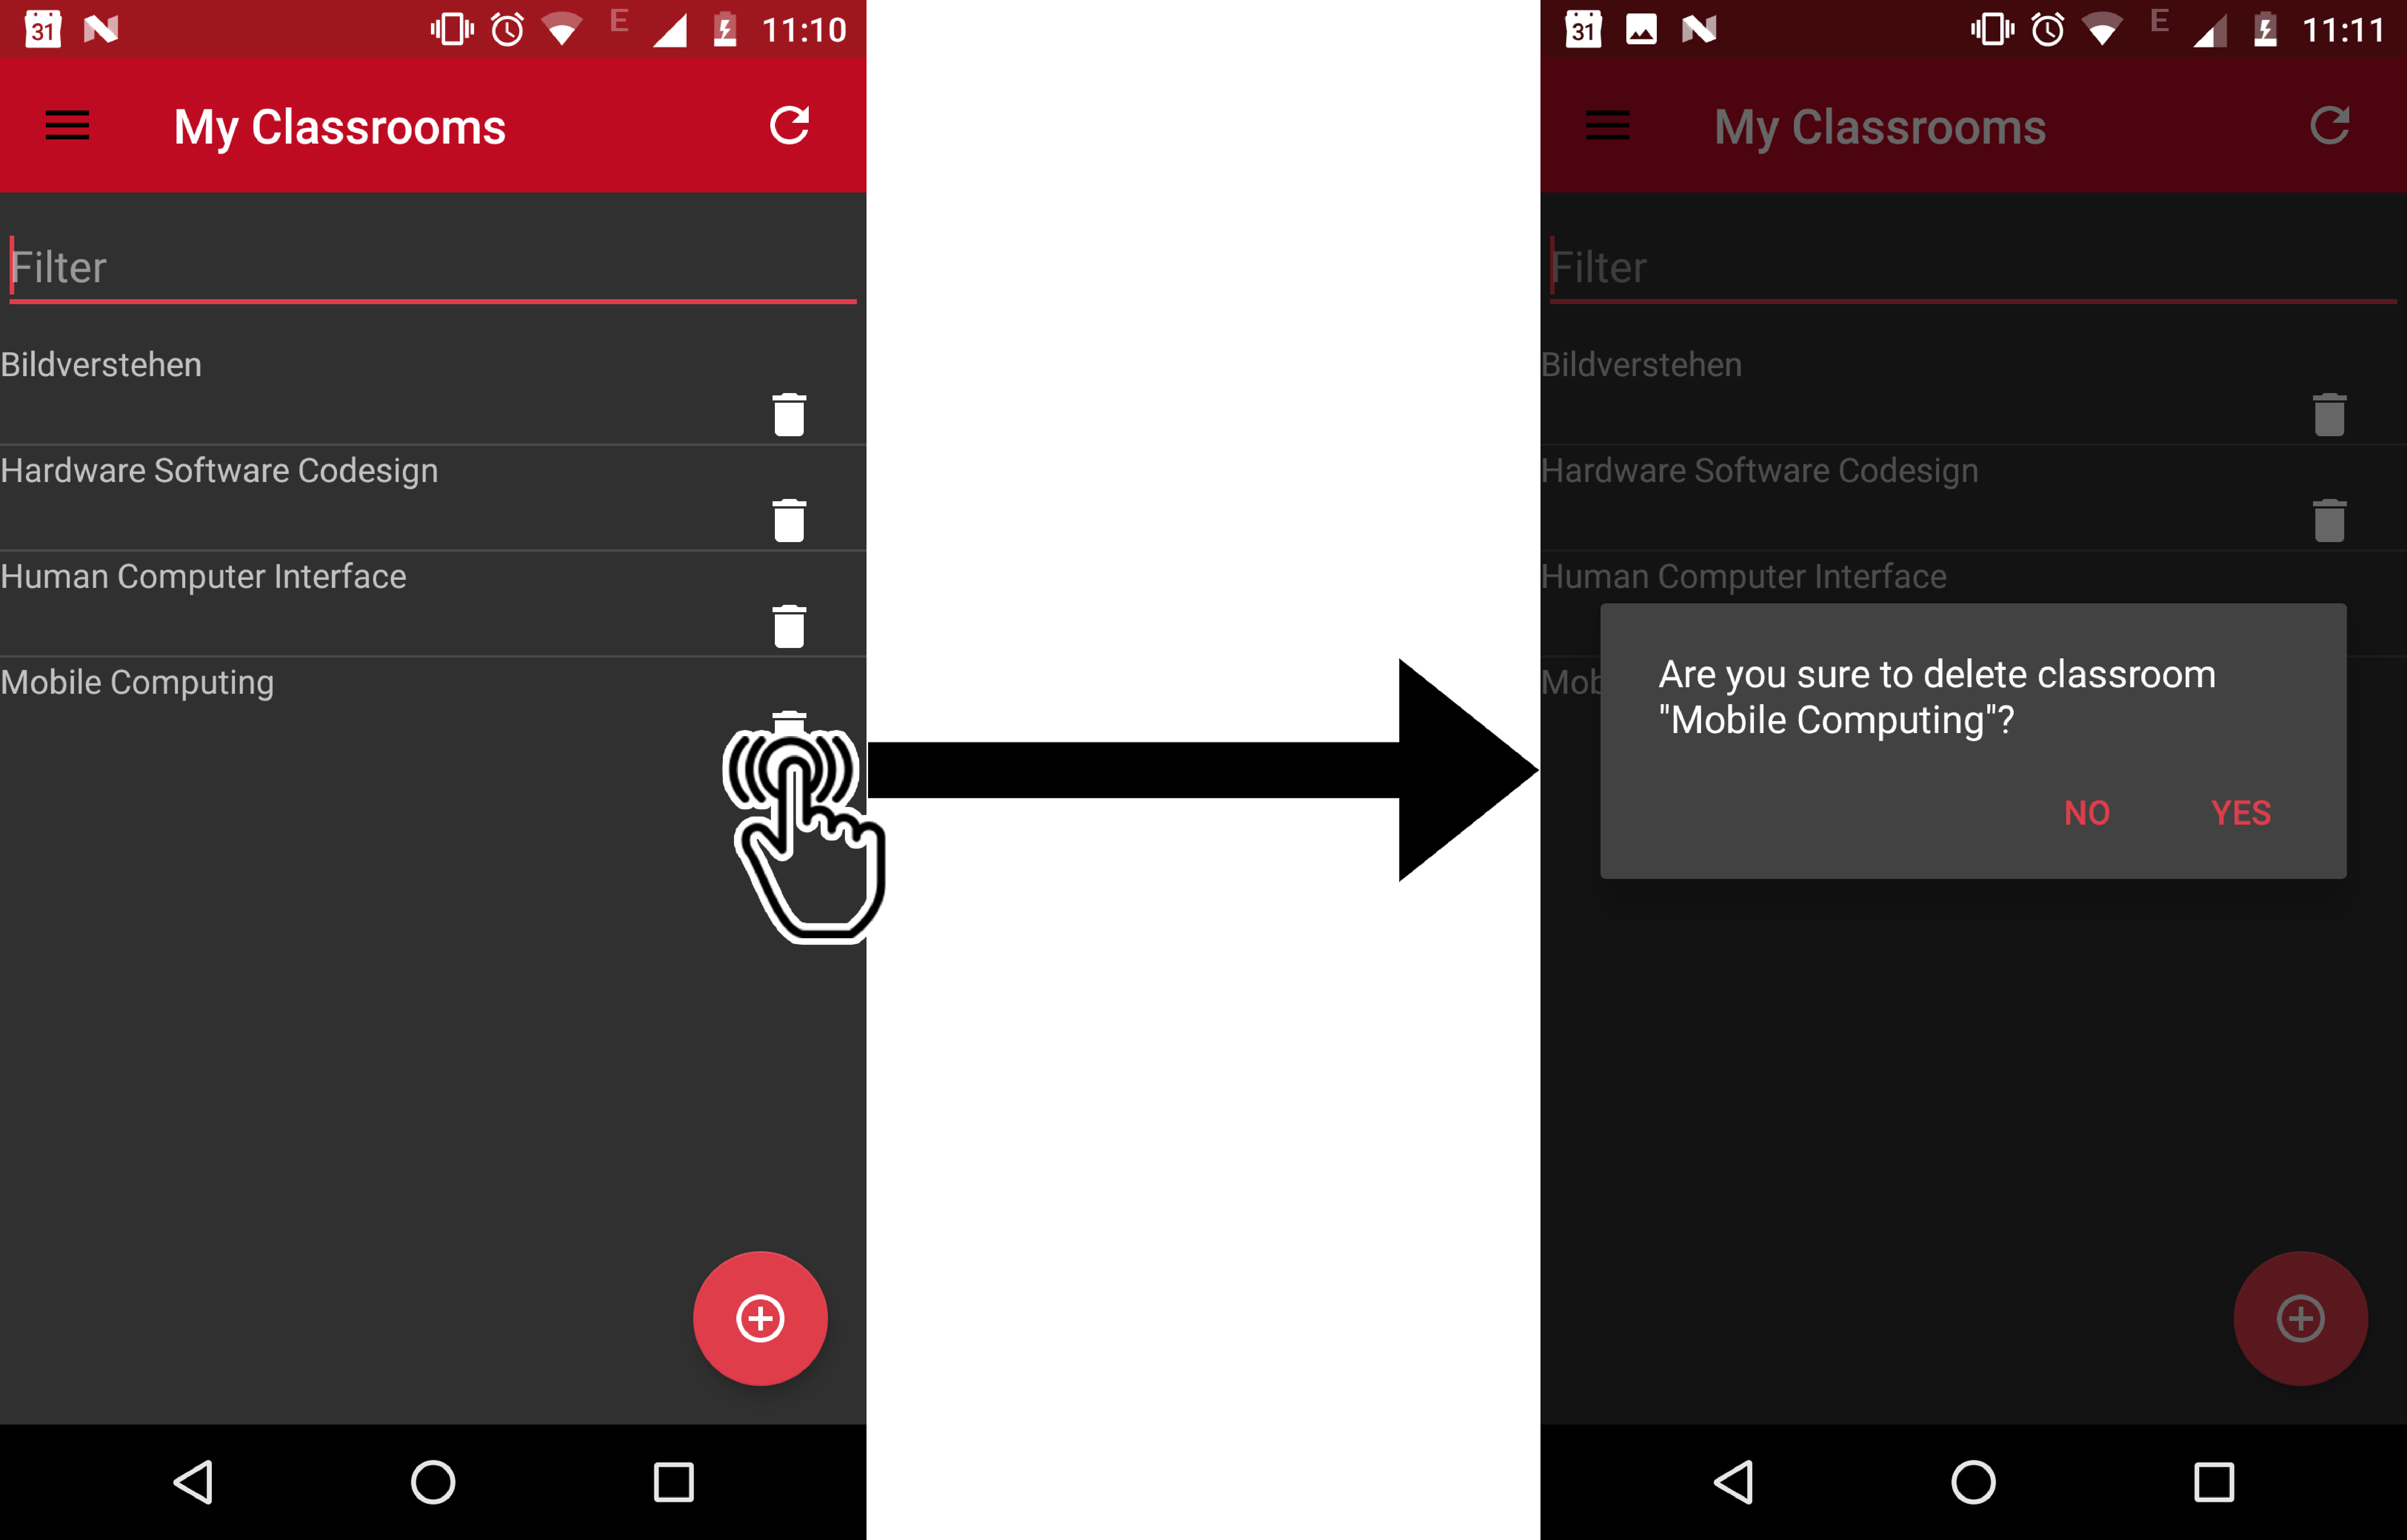
\includegraphics[scale=0.10]{Resources/LecturerMyClassrooms}
	\caption{Löschen eines Kursraums für Benutzer in der Rolle \enquote{Dozent}}
	\label{pic:LecturerDeleteClassroom}
	\end{center}
\end{figure}

\begin{figure}[H]
	\begin{center}
	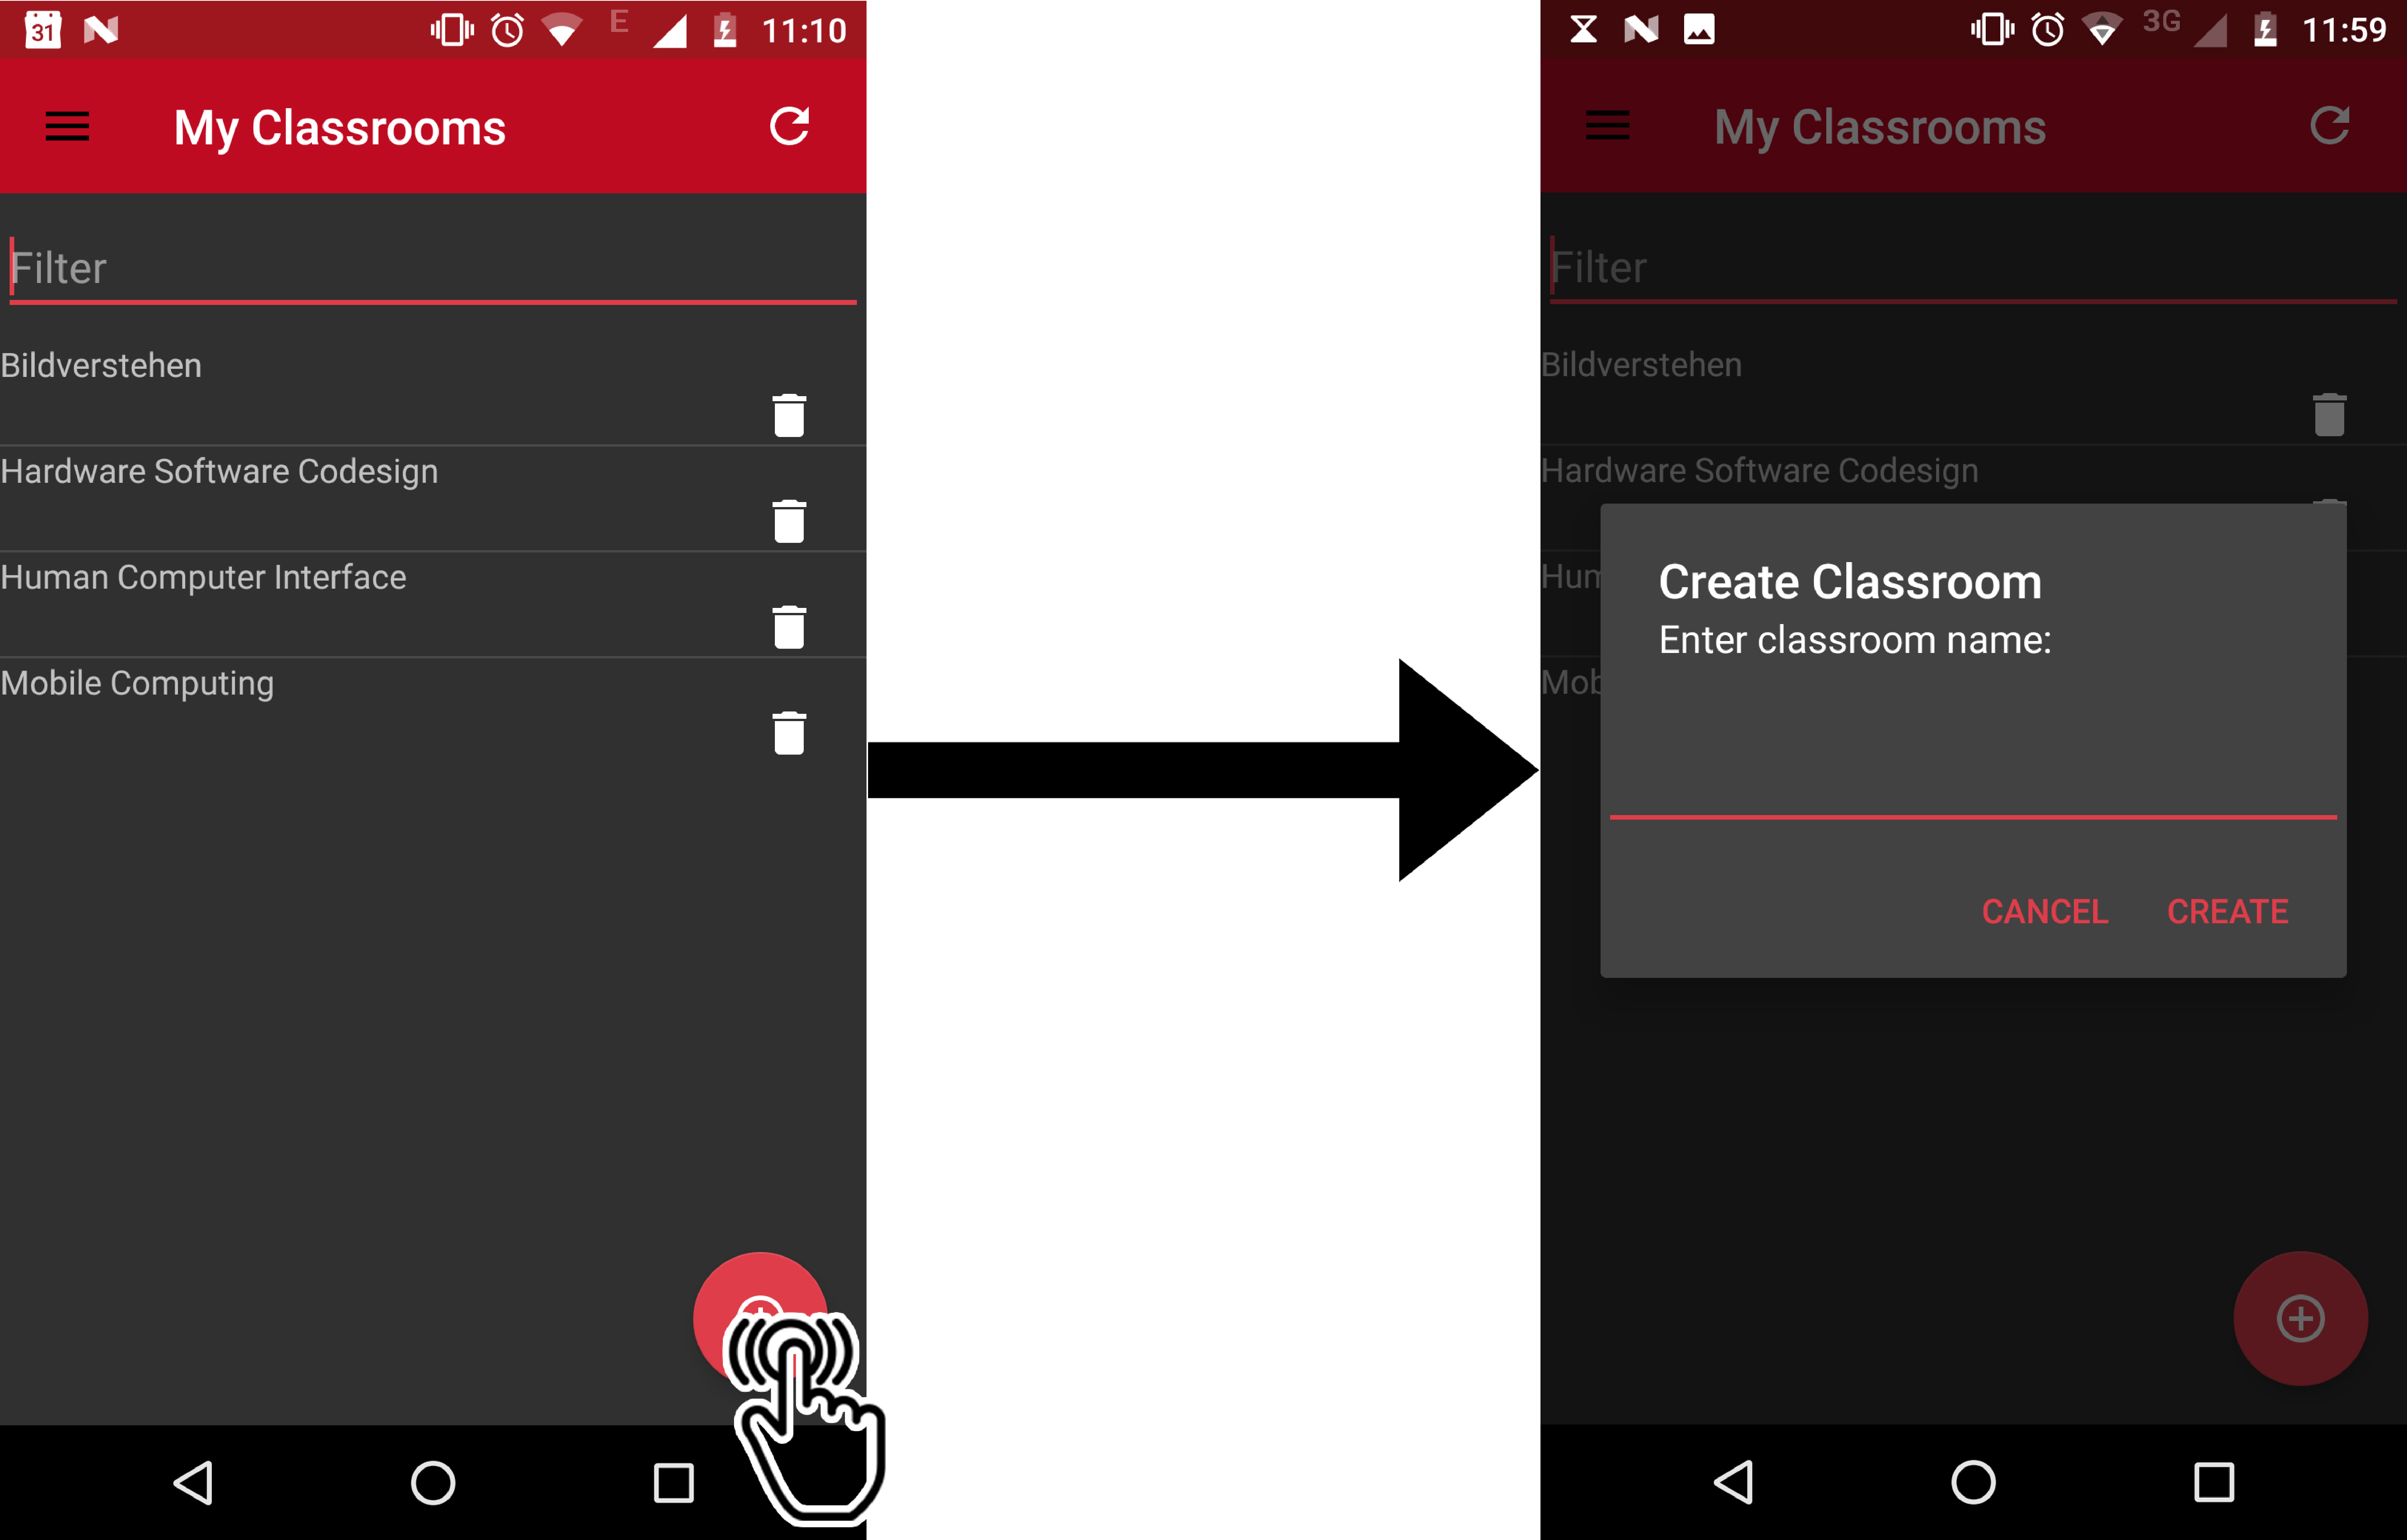
\includegraphics[scale=0.10]{Resources/LecturerCreateClassroom}
	\caption{Erstellen eines Kursraums in der Rolle \enquote{Dozent}}
	\label{pic:LecturerCreateClassroom}
	\end{center}
\end{figure}

Durch Klicken auf den Namen eines Kursraums wird in die Übersichtansicht für den gewählten Kursraum 
(siehe Abbildung \ref{pic:LecturerClassroom}).
Es werden nun alle Nachrichten angezeigt, die der Dozent in der Vergangenheit in den Kursraum eingestellt hat.
Nun besteht die Möglichkeit eine neue Nachricht zu erstellen.
Hierfür muss der \enquote{erstellen}-Button in der Ansicht unten rechts gedrückt werden.
Nun erscheint ein Dialog, in dem der Inhalt der neuen Nachricht eingegeben werden kann.
Mit \enquote{Okay} wird das Erstellen der Nachricht bestätigt; sie ist nun für alle Studenten, die diesen Kursraum abonniert haben sichtbar.
Für genaueres Verständnis ist der Ablauf dieser Benutzerinteraktion in Abbildung \ref{pic:LecturerPostMessage} dargestellt.
Möchte der Dozent eine Nachricht aus dem Kursraum entfernen, so betätigt er den \enquote{Löschen} Button neben der betreffenden Nachricht. 
Nun erscheint ein Dialog, der den Benutzer zu erneutem Bestätigten der Löschung aufruft.
Bestätigt der Anwender mit der Option \enquote{Delete} so wird die Nachricht gelöscht.
\begin{figure}[H]
	\begin{center}
	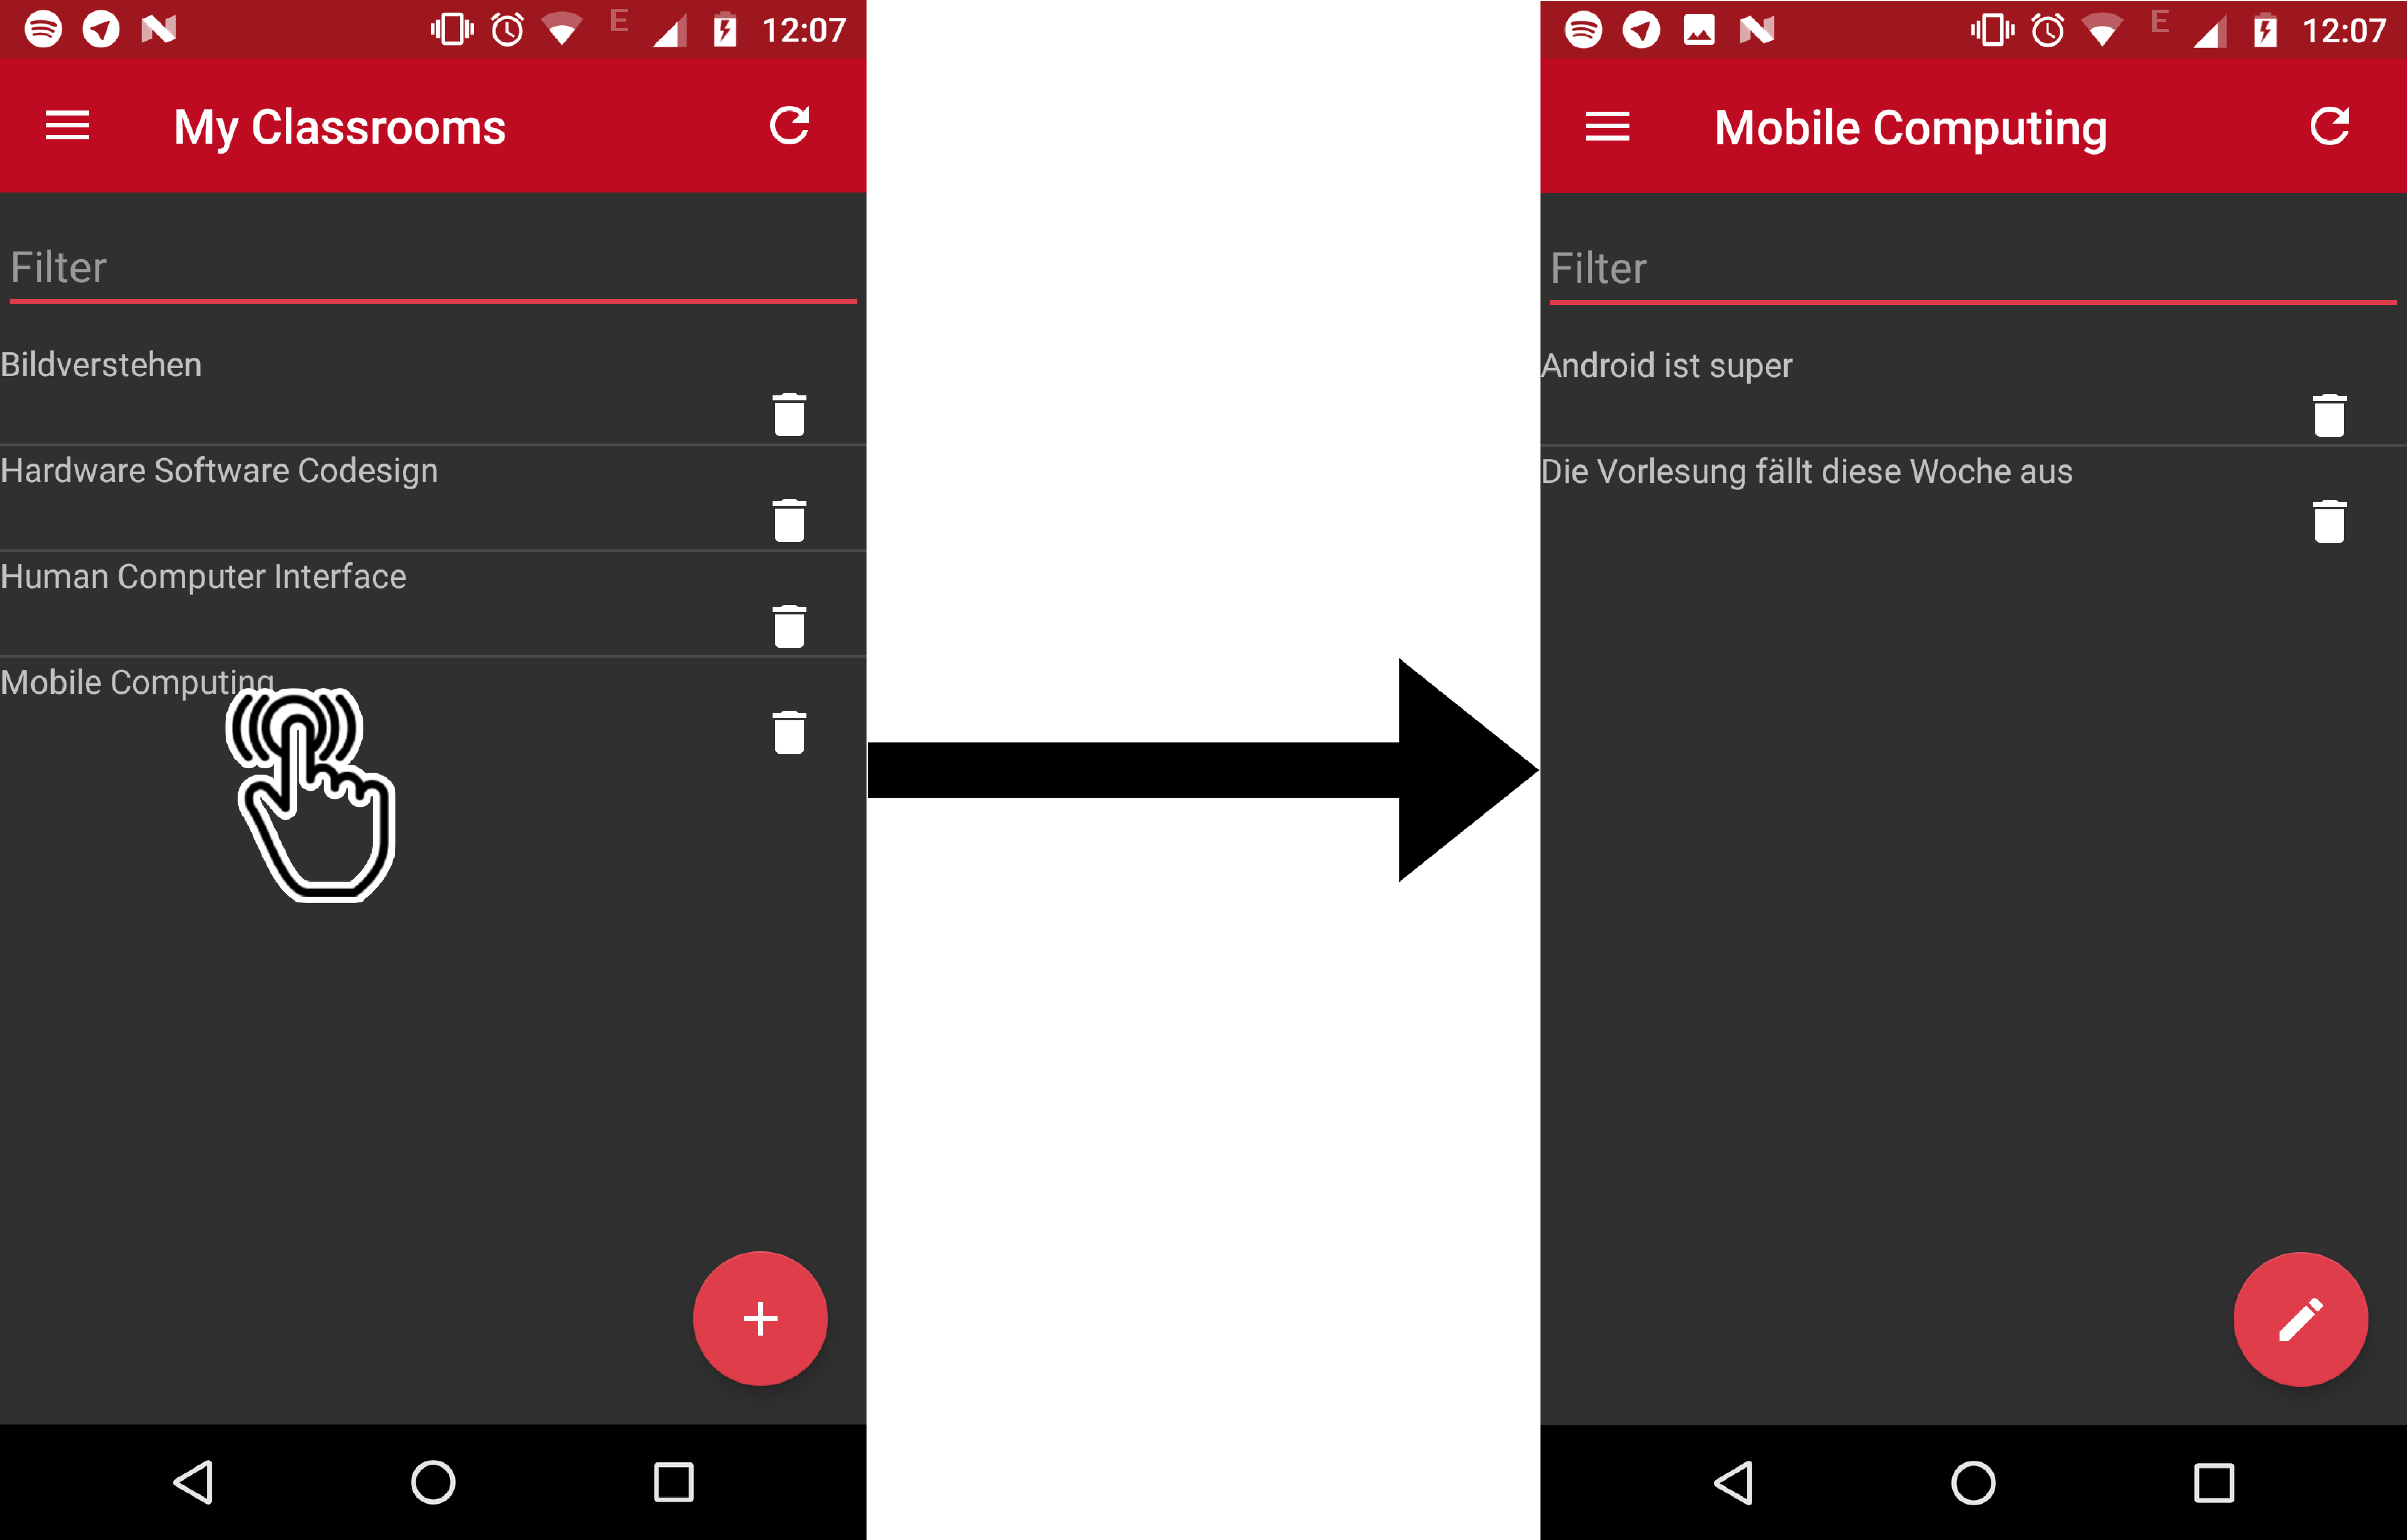
\includegraphics[scale=0.10]{Resources/LecturerClassroom}
	\caption{Wechseln zur Übersicht über einen Kursraum für Benutzer in der Rolle \enquote{Dozent}}
	\label{pic:LecturerClassroom}
	\end{center}
\end{figure}

\begin{figure}[H]
	\begin{center}
	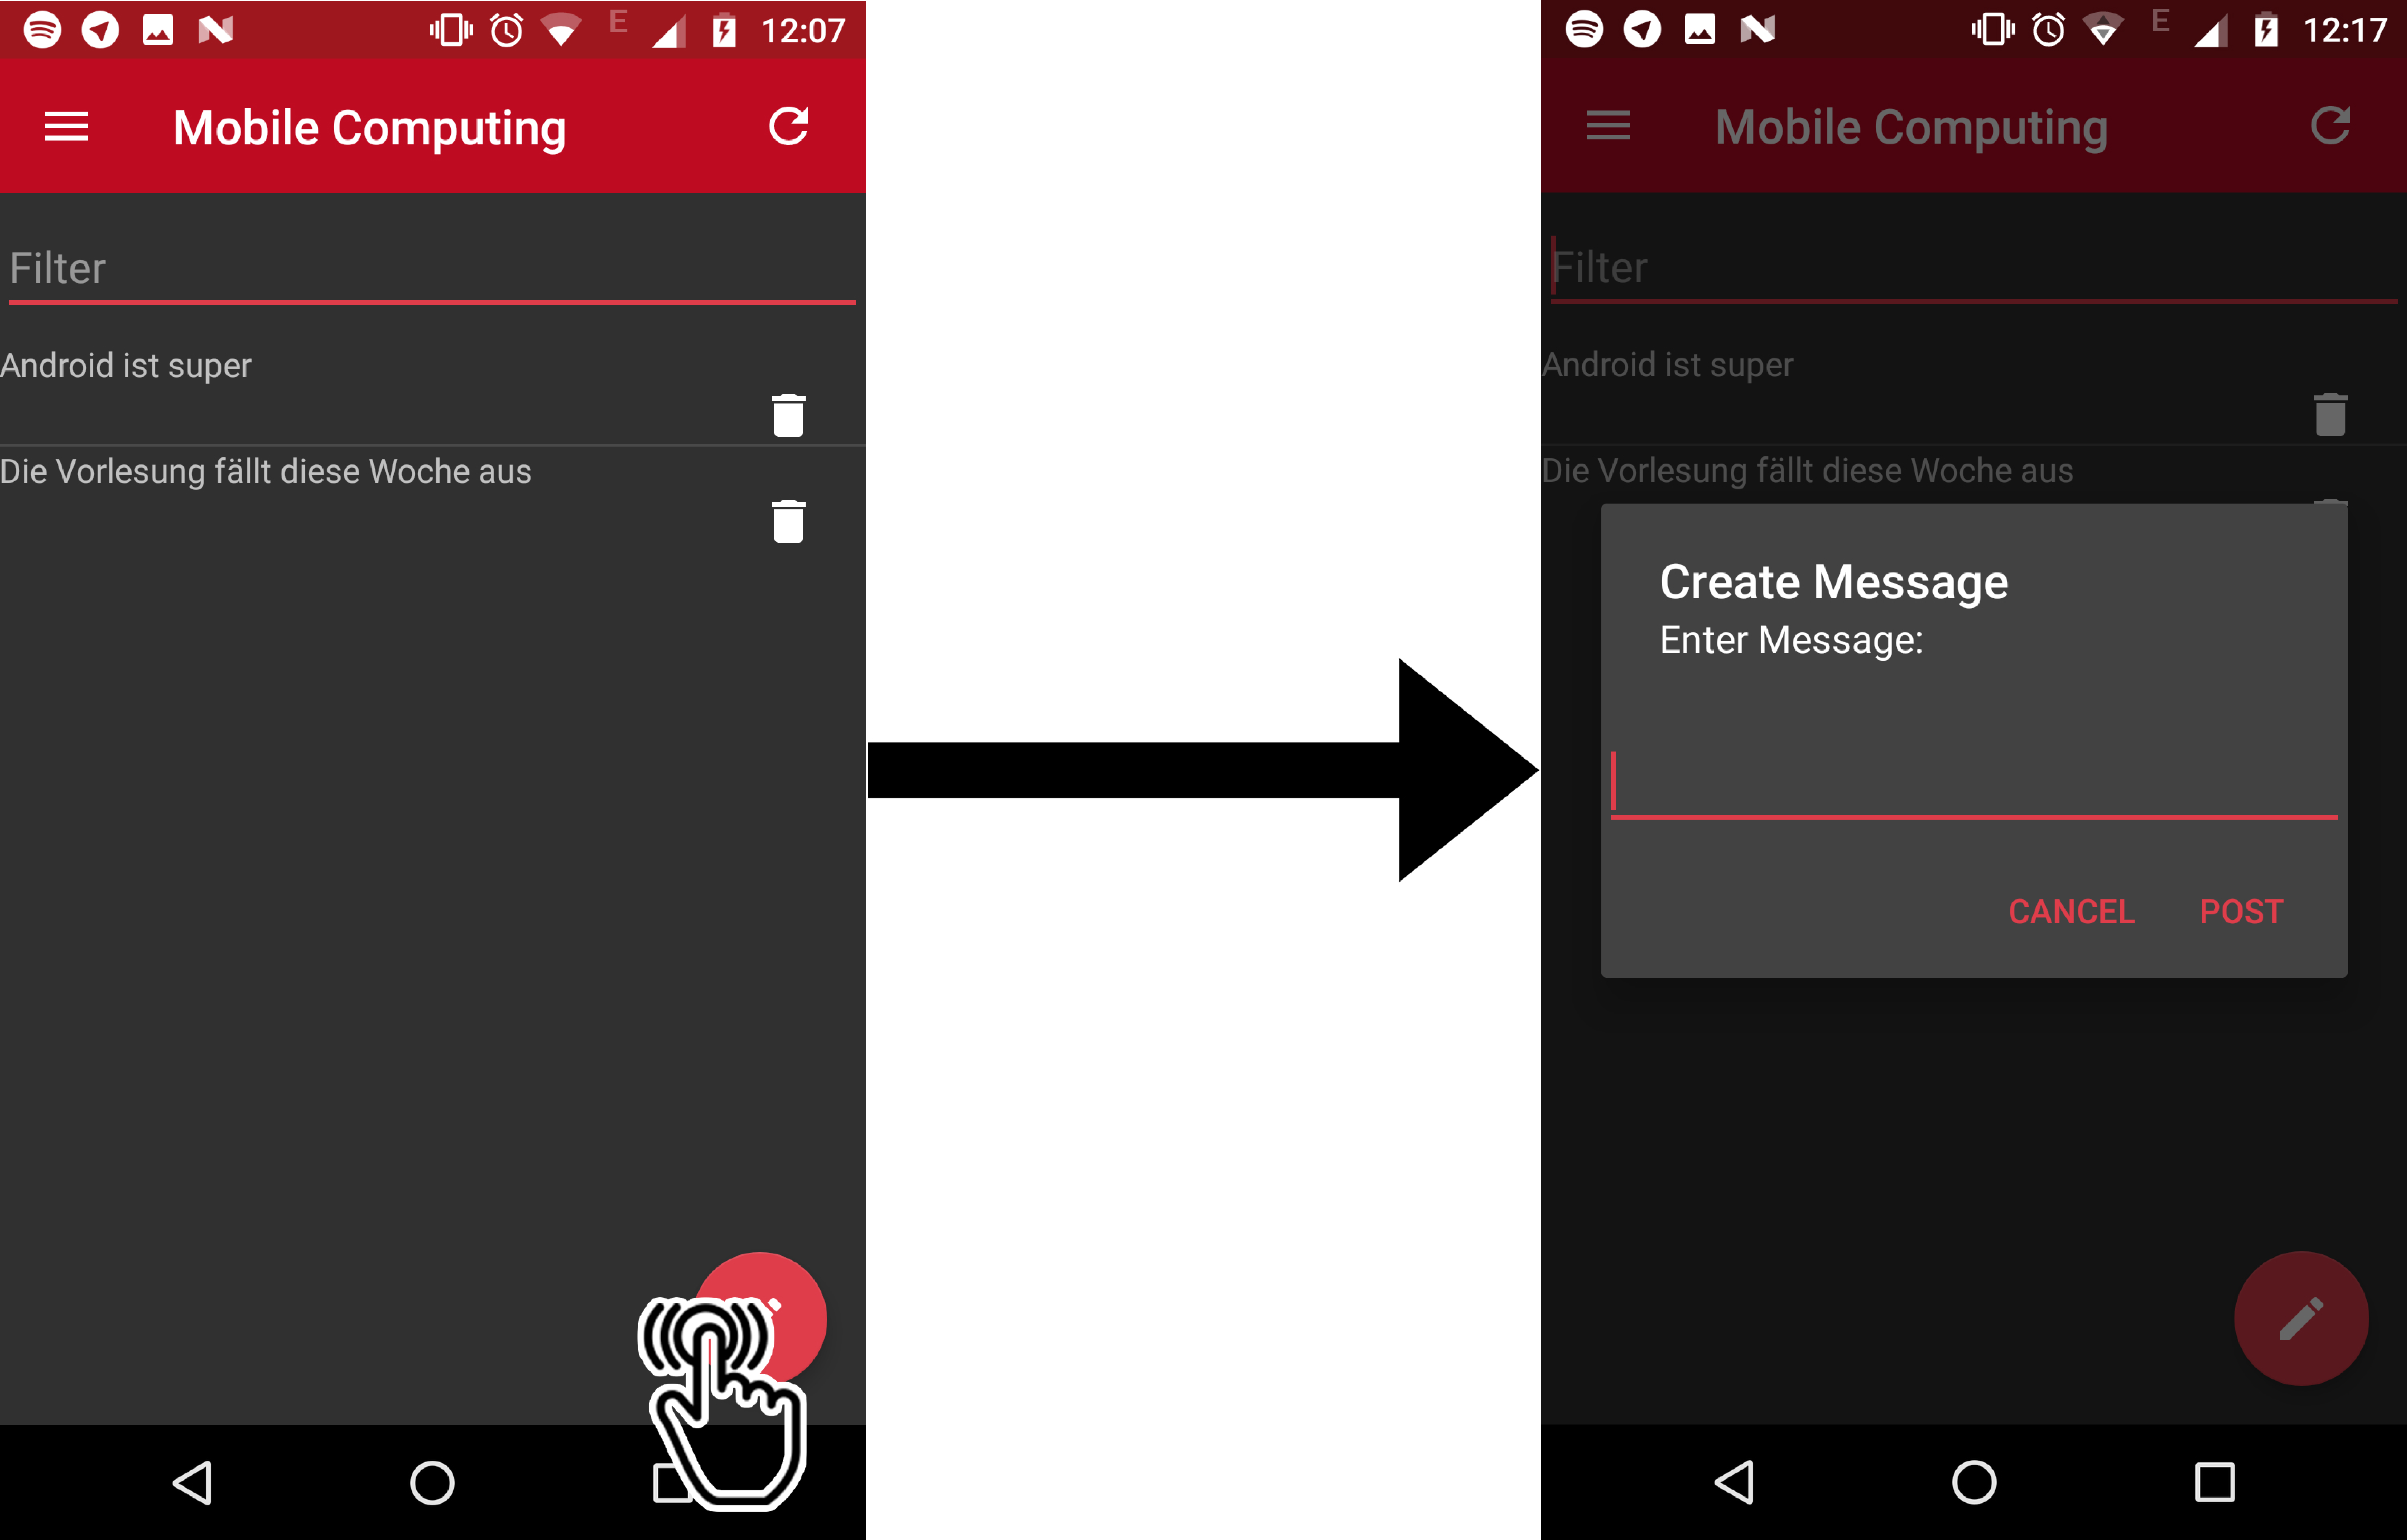
\includegraphics[scale=0.10]{Resources/LecturerPostMessage}
	\caption{Einstellen einer Nachricht in einem Kursraum für Benutzer in der Rolle \enquote{Dozent}}
	\label{pic:LecturerPostMessage}
	\end{center}
\end{figure}

\begin{figure}[H]
	\begin{center}
	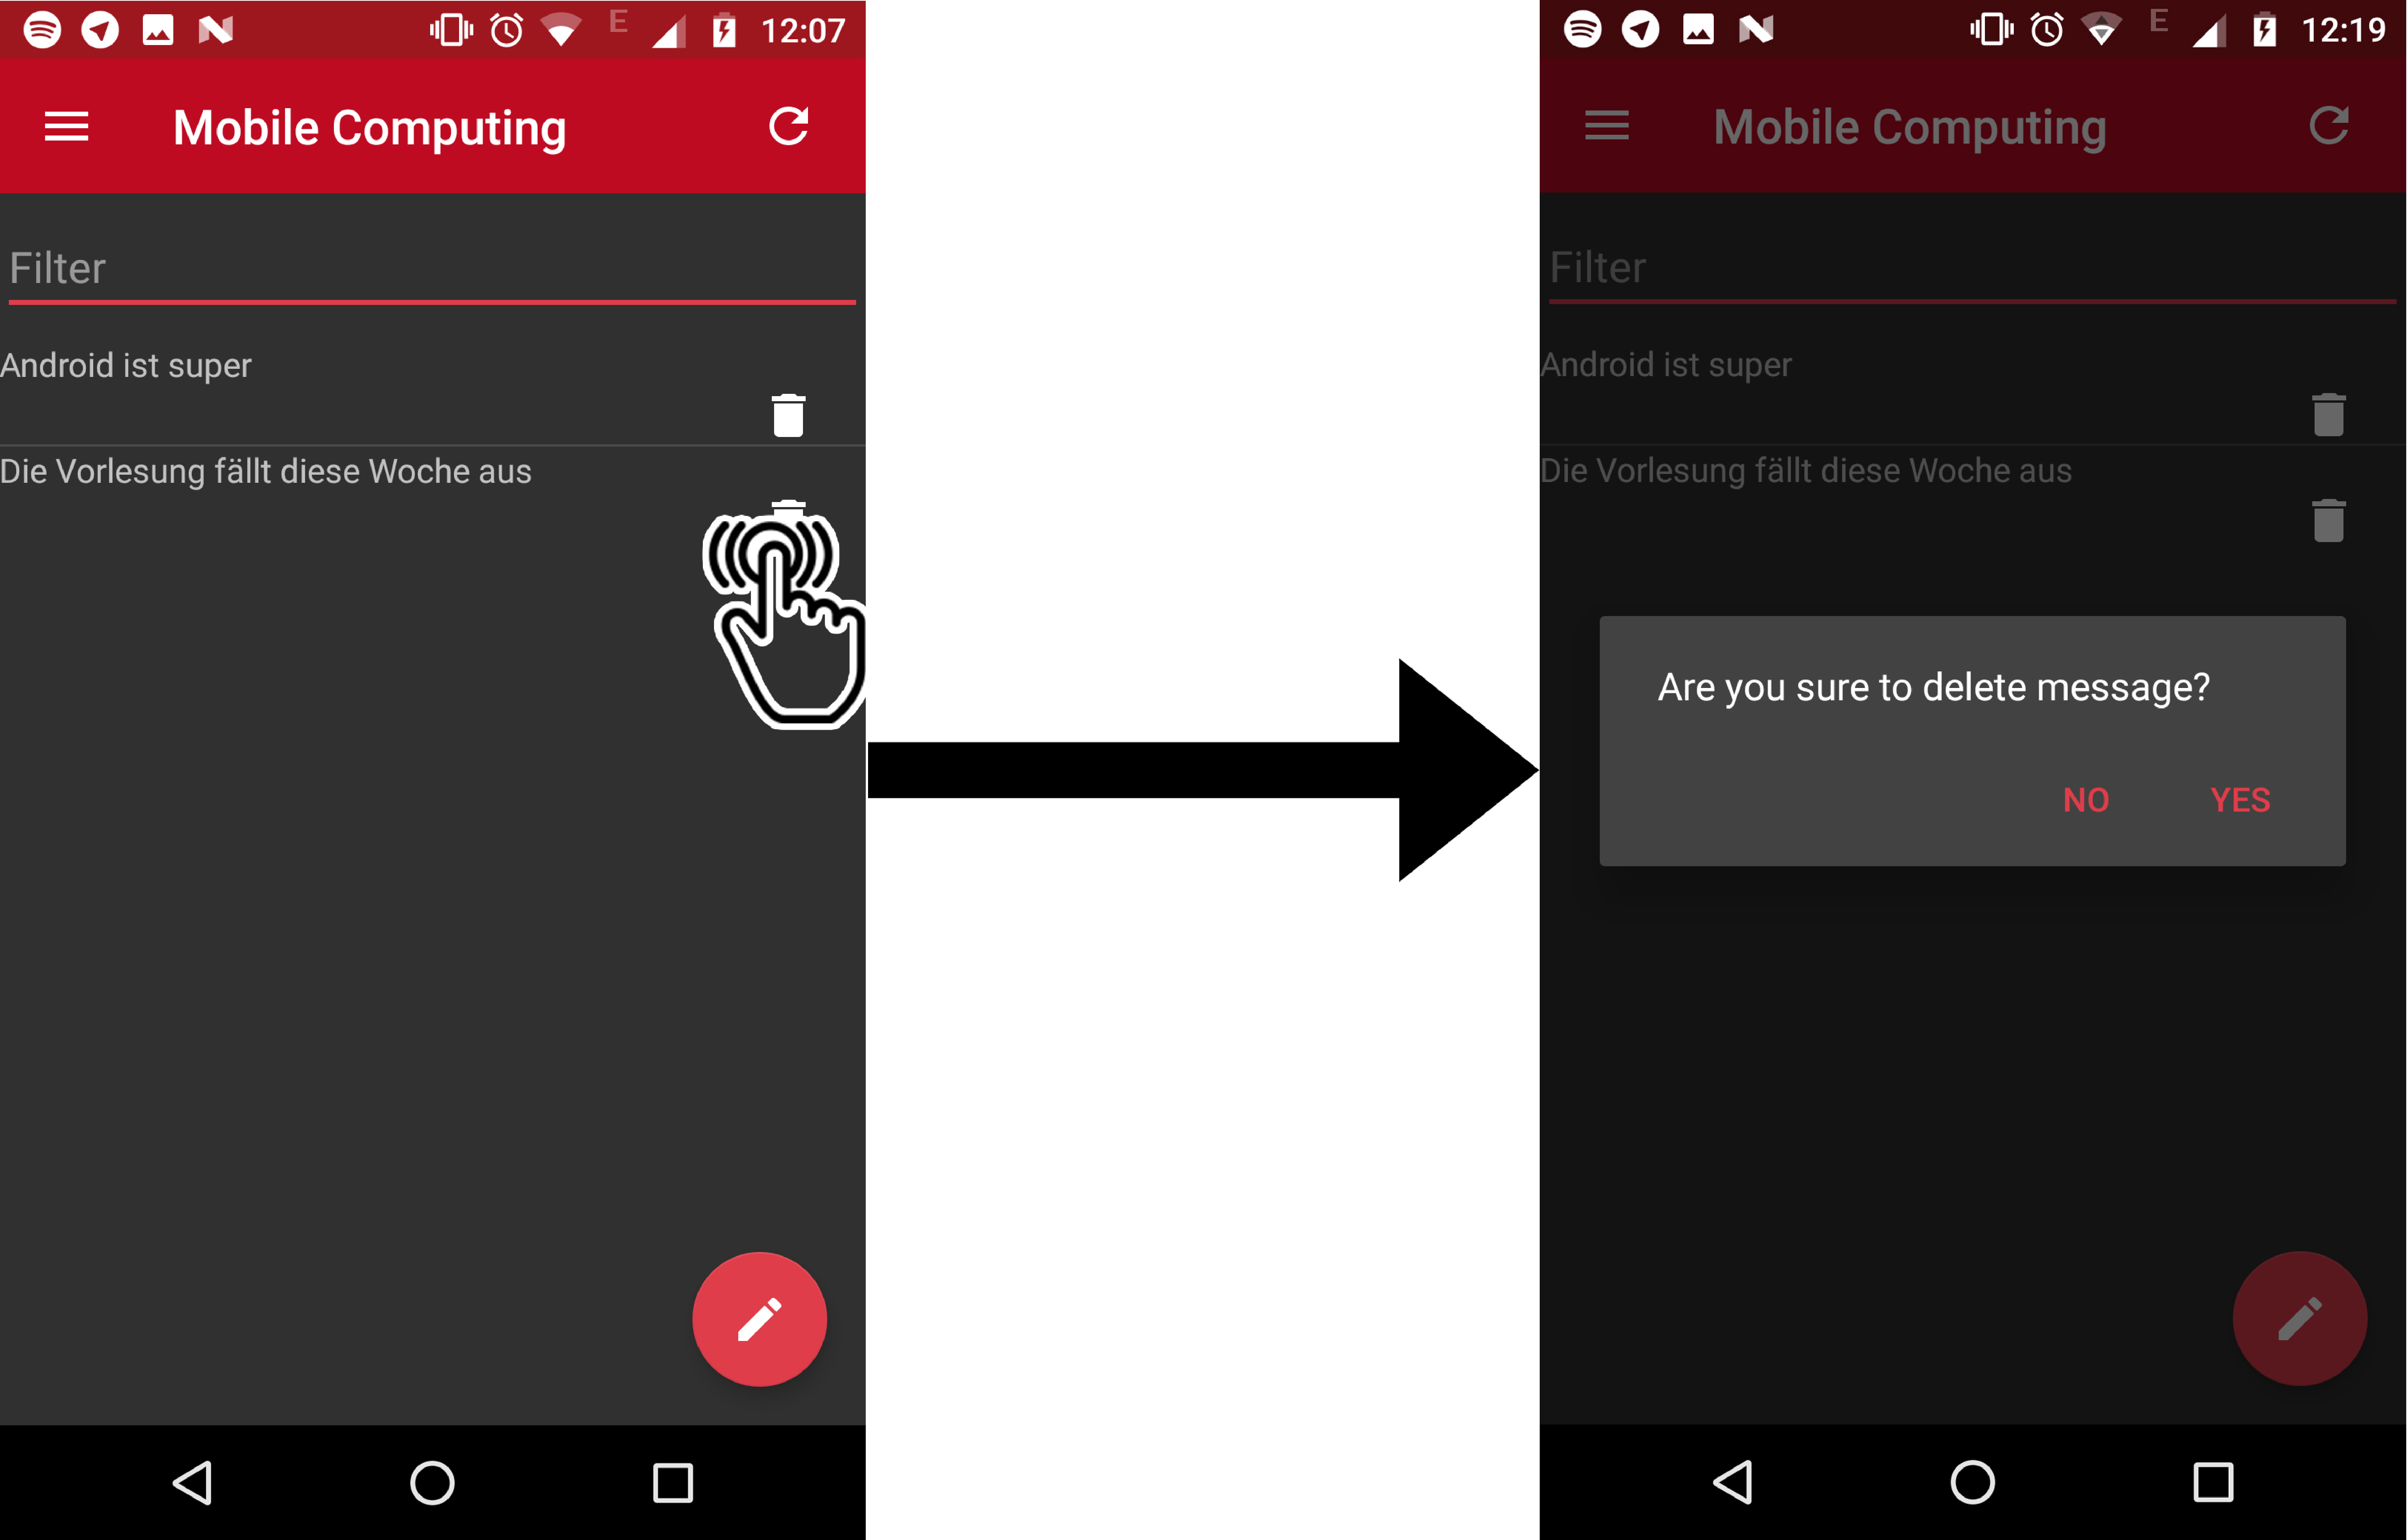
\includegraphics[scale=0.10]{Resources/LecturerDeleteMessage}
	\caption{Löschen einer Nachricht in einem Kursraum für Benutzer in der Rolle \enquote{Dozent}}
	\label{pic:LecturerDeleteMessage}
	\end{center}
\end{figure}



\newpage
\subsection{Oberfläche für Studenten}\label{section:StudentenOberflache}
Nach erfolgreicher Anmeldung wird einem Studenten die Oberfläche aus Abbildung \ref{pic:StudentenMyMessages} gezeigt. Hier werden alle Nachrichten aus seinen abonnierten Kursräumen -- sortiert nach Einstellzeitpunkt -- angezeigt.
Die angezeigten Daten werden sofort nach betreten dieser Ansicht vom Server geladen.
Durch Drücken auf das \enquote{Refresh} Symbol oben rechts, werden die Nachrichten erneut vom Server abgerufen und eventuell zwischenzeitlich neu eingestellte ebenfalls angezeigt.
Der Menü-Button oben links führt den Benutzer in die Ansicht aus Abbildung \ref{pic:StudentenOberflache}.
Zur Verbesserung der Übersichtlichkeit kann in dem Texteingabefeld \enquote{Filter} ein Suchtext eingegeben werden; es werden so nur noch Nachrichten angezeigt, deren Kursraum oder Nachrichtentext die eingegebene Zeichenfolge enthält.
\begin{figure}[H]
	\begin{center}
	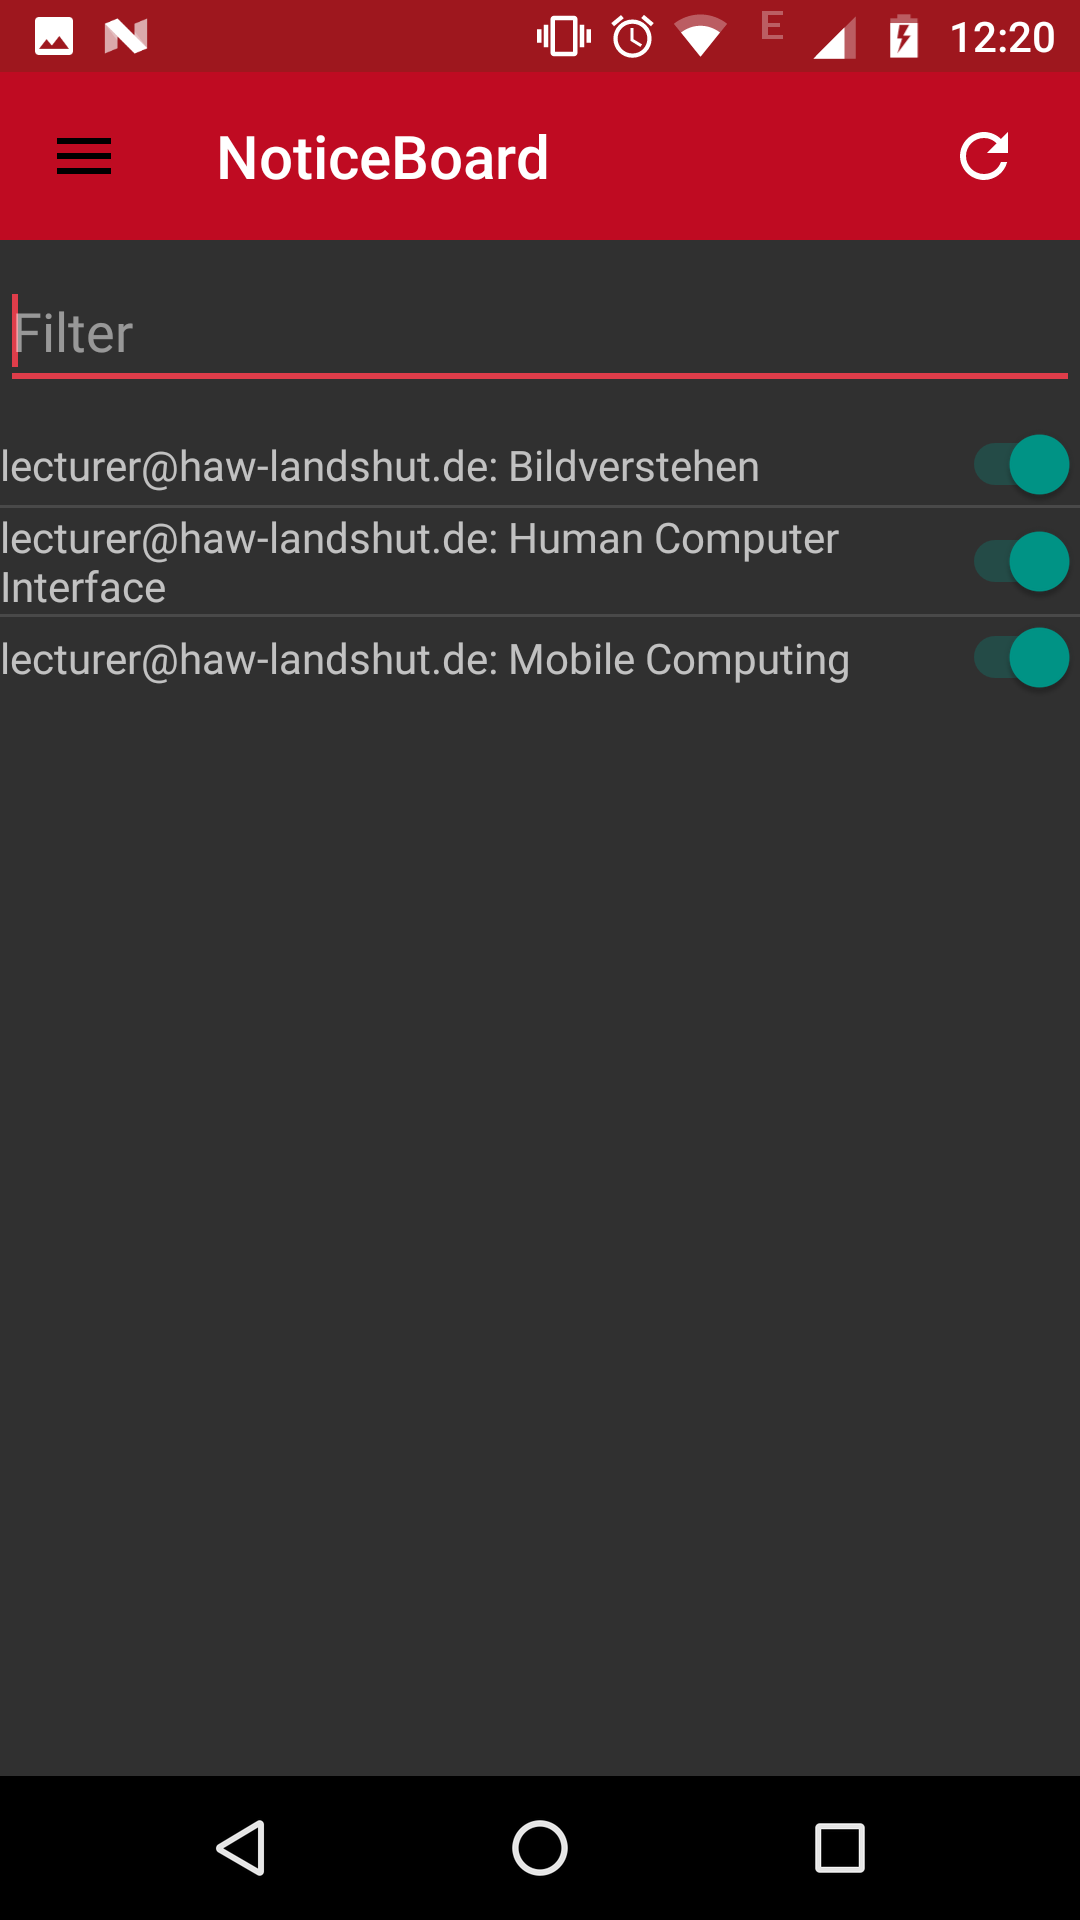
\includegraphics[scale=0.1]{Resources/ActivityMyClassrooms}
	\caption{Hauptmenü für Benutzer in der Rolle \enquote{Student}}
	\label{pic:StudentenMyMessages}
	\end{center}
\end{figure}

Studenten können mittels des in Abbildung \ref{pic:StudentenOberflache} gezeigtem Screens durch die App navigieren.
Es können mit \enquote{My Messages} alle aktuellen Nachrichten der abonnierten Kursräume angezeigt werden. 
Unter \enquote{My Classrooms} werden alle abonnierten Klassenräume geladen, diese können hier deabonniert werden.
Über die Option \enquote{All Classrooms} werden alle offenen Kursräume angezeigt; ein Student hat so die Möglichkeit diese zu abonnieren beziehungsweise zu deabonnieren.
Über den Menüpunkt \enquote{logout} meldet sich der Anwender aus der Applikation ab und gelangt zurück in die Authentifizierungsansicht.
\begin{figure}[H]
	\begin{center}
	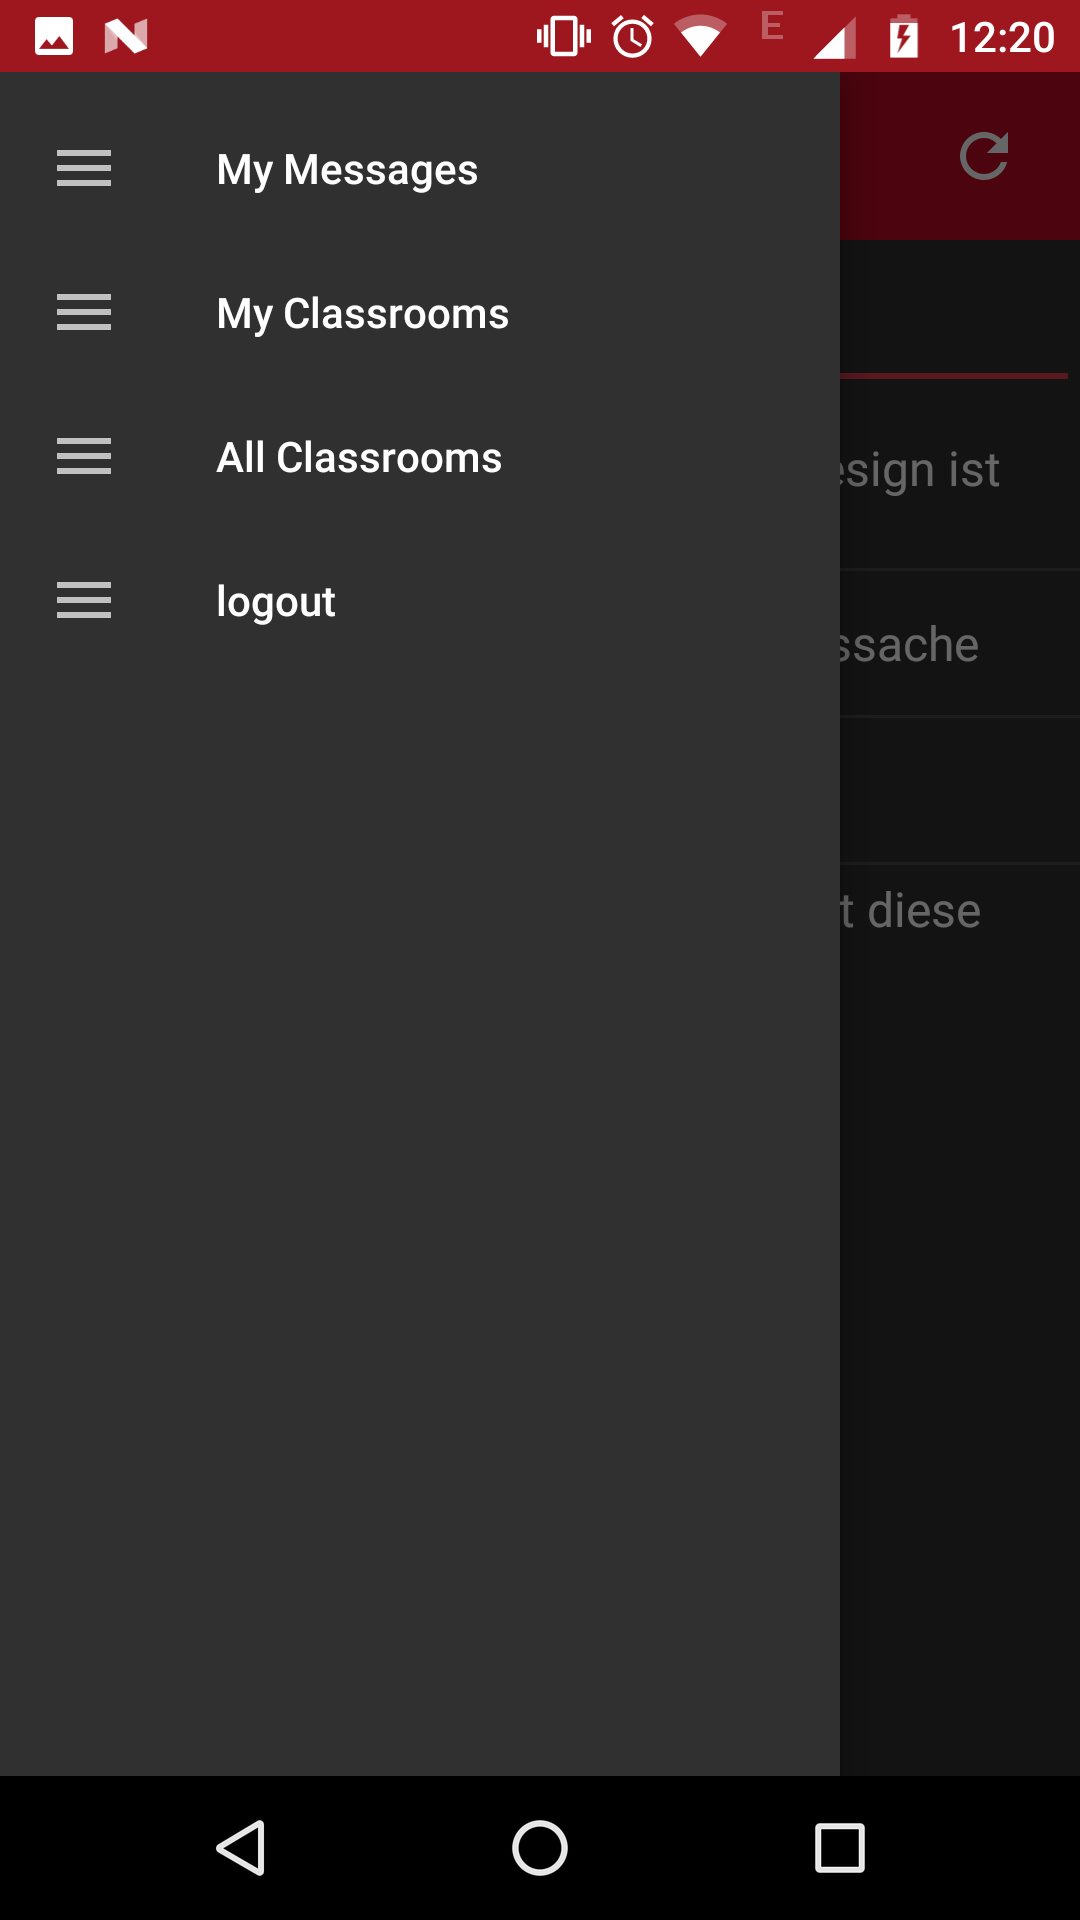
\includegraphics[scale=0.10]{Resources/ActivityMainMenuStudent}
	\caption{Hauptmenü für Benutzer in der Rolle \enquote{Student}}
	\label{pic:StudentenOberflache}
	\end{center}
\end{figure}
\newpage
In der Ansicht, die in Abbildung \ref{pic:StudentenMyClassrooms} dargestellt ist, werden Benutzern in der Rolle \enquote{Student} alle Kursräume und der zugeordnete Dozent angezeigt, die sie abonniert haben.
Rechts neben jedem abonnierten Kursraum befindet sich ein Schalter, der anzeigt, ob der betreffende Klassenraum abonniert ist oder nicht. 
Bei Betreten der Ansicht werden alle Kursräume als abonniert markiert. 
Durch Betätigen des Schalters wird der entsprechende Kursraum deabonniert und der Schalter steht auf aus. 
Es besteht die Möglichkeit durch erneutes Drücken den Kursraum wieder zu abonnieren; erst bei manueller Aktualisierung mittels des \enquote{Refresh}-Symbols wird der Kursraum entfernt. 
Filtern analog zur Oben beschriebenen Oberfläche ist ebenfalls möglich.
\begin{figure}[H]
	\begin{center}
	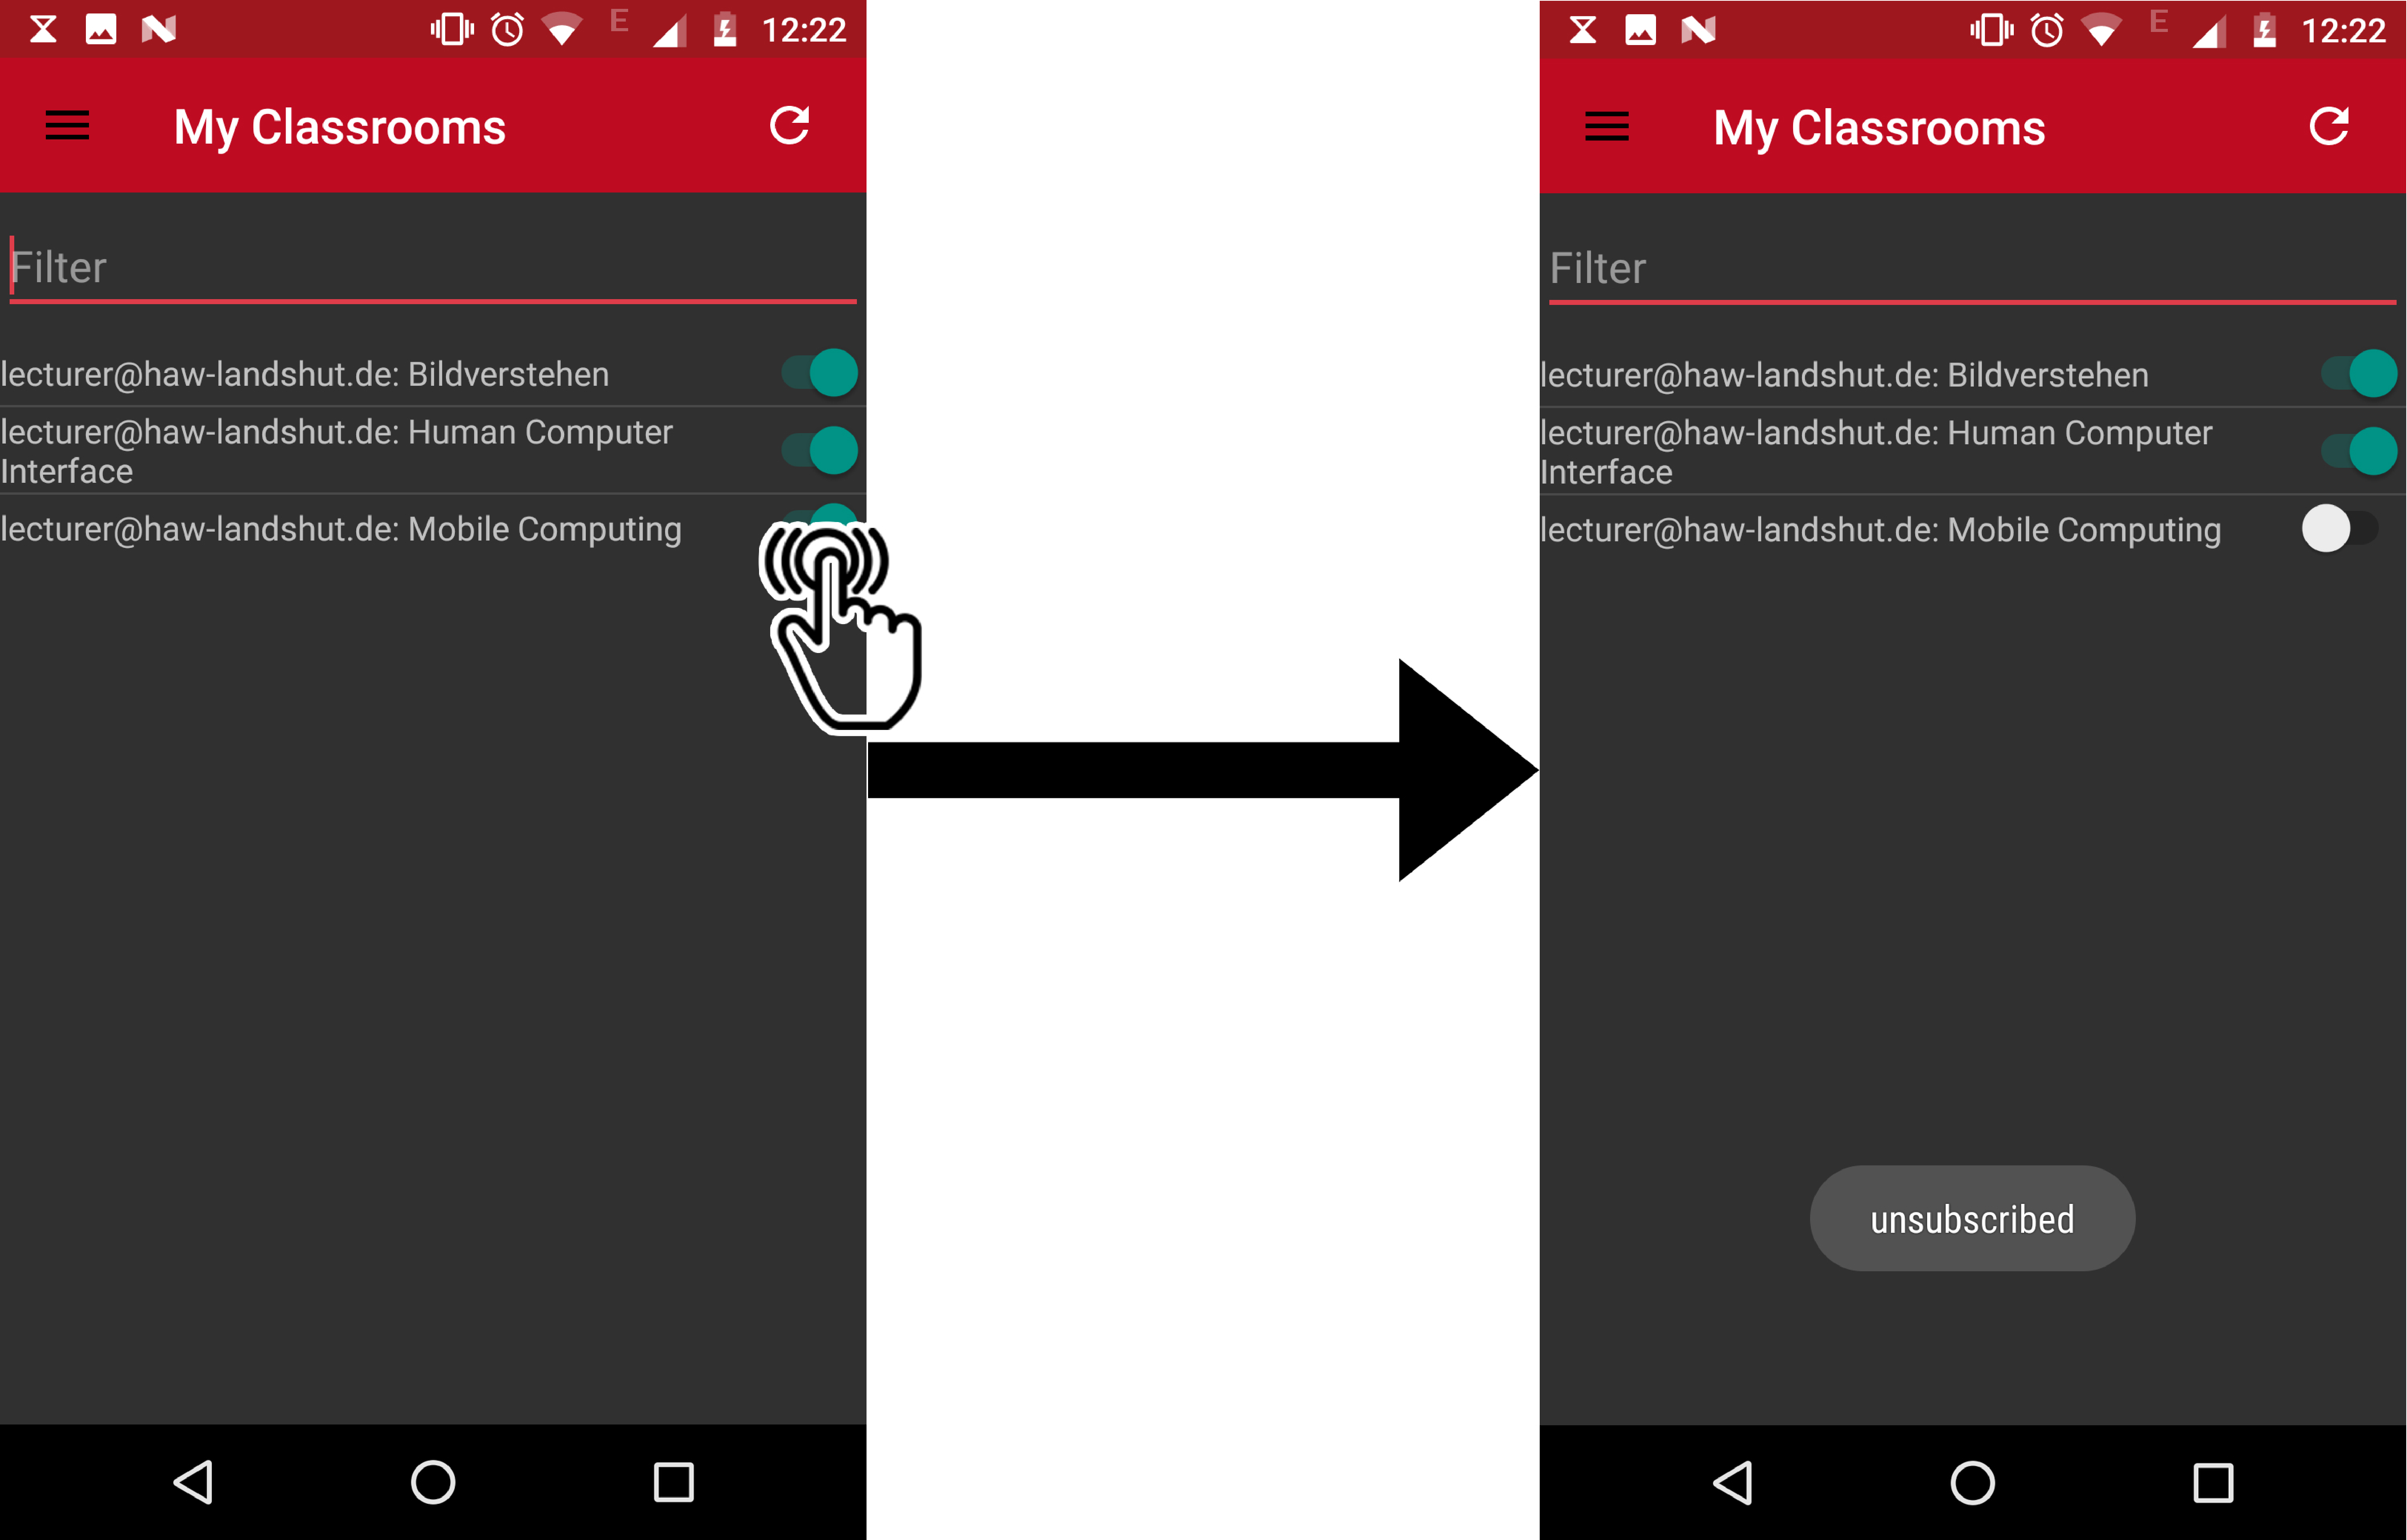
\includegraphics[scale=0.10]{Resources/StudentUnsubscribeClassroom}
	\caption{Deabonnieren eines Kursraums für Benutzer in der Rolle \enquote{Student}}
	\label{pic:StudentenMyClassrooms}
	\end{center}
\end{figure}

Die Activity \enquote{All Classrooms} (Abbildung \ref{pic:StudentenAllClassrooms}) zeigt alle Kursräume, die vom Benutzer abonniert werden können. Nicht abonnierte Kursräume werden mit einem deaktiviertem Schalter markiert und umgekehrt.
Der Anwender hat hier die Möglichkeit weitere Kursräume zu suchen und abonnieren oder gegebenenfalls auch zu de-abonnieren.
Bei Betreten dieser Activity werden die aktuellen Daten vom Server abgerufen, Betätigen des \enquote{Refresh}-Symbols aktualisiert die Daten manuell.
Über das Menü Symbol gelangt der Benutzer zurück in die Navigation.
\begin{figure}[H]
	\begin{center}
	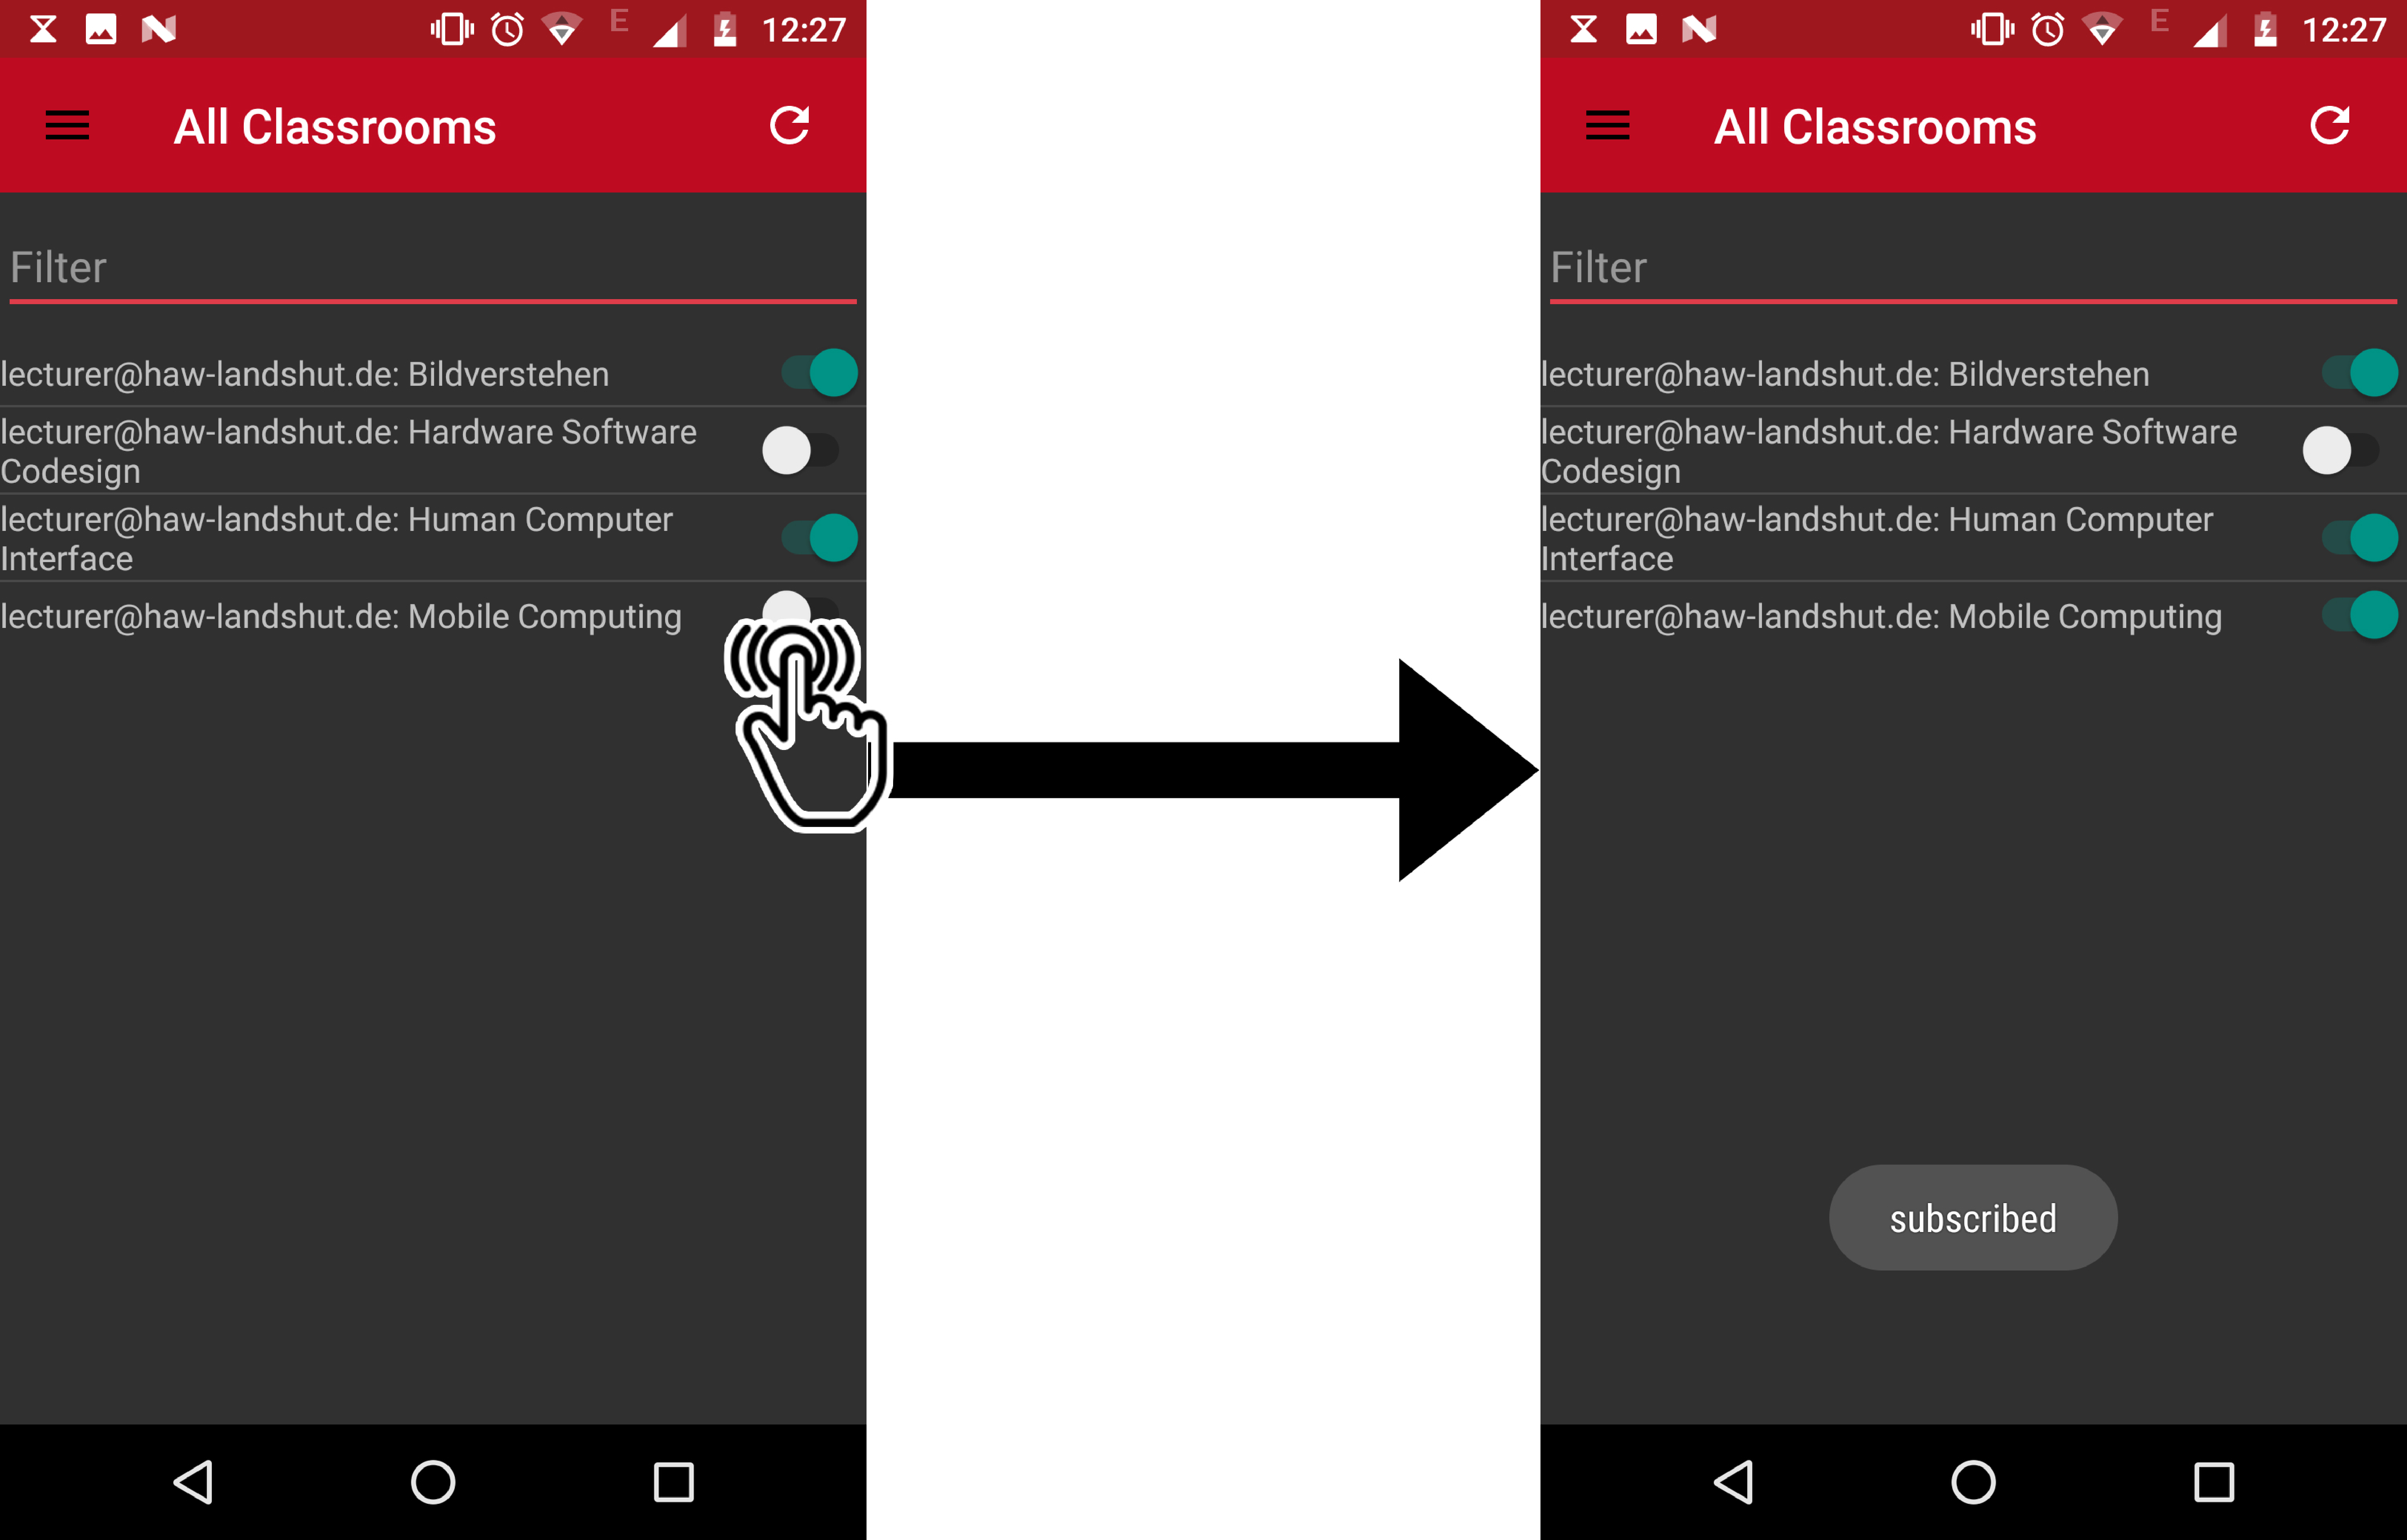
\includegraphics[scale=0.10]{Resources/StudentSubscribeClassroom}
	\caption{Abonnieren eines Kursraums für Benutzer in der Rolle \enquote{Student}}
	\label{pic:StudentenAllClassrooms}
	\end{center}
\end{figure}
\newpage
\section{Backend}
Damit die Nutzer der App interaktiv miteinander kommunizieren können, ist eine Verbindung zu einem Server (im weiteren als Backend bezeichnet) nötig.
Daten wie Klassenräume und Nachrichten können unter Angabe von validen Anmeldedaten abgefragt werden.
Als Schnittstelle zwischen der App und dem Backend findet eine REST-API Verwendung.
Die Datenbank verwaltet alle Daten wie Klassenräume, eingestellte Nachrichten und Anmeldedaten.
Eine Grundsätzliche Struktur der Architektur der Komposition von SQL-Datenbank, REST-API und App ist in Abbildung \ref{pic:backendArchitektur} dargestellt.
\begin{figure}[H]
	\begin{center}
	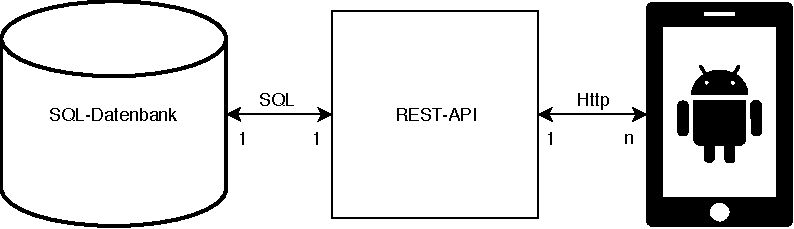
\includegraphics[scale=0.8]{Resources/BackendArchitektur}
	\caption{Architektur des Backends}
	\label{pic:backendArchitektur}
	\end{center}
\end{figure}
\subsection{Datenbank}
Zur Verwaltung der Anmeldedaten, Klassenräume, Nachrichten und Abonnements wird eine relationale Datenbank eingesetzt.
Die Tabelle \enquote{Persons} enthält die Anmeldedaten (E-Mailadresse und Passwort) jedes Nutzers, sowie dessen jeweilige Rolle (Student, Dozent, Admin).
In \enquote{Messages} sind die Nachrichten gespeichert, die Dozenten in ihre Kursräume einstellen. Jede Nachricht ist einem Kursraum eindeutig zugeordnet und erhält eine eindeutige id. Im Feld \enquote{Payload} ist der eigentliche Text der Nachricht abgespeichert.
Kursraum werden in der Tabelle \enquote{Classrooms} verwaltet.
Jedem Raum ist ein Dozent eindeutig zugeordnet.
Über die \enquote{subscribes} wird die n:m-Beziehung zwischen Studenten und Kursräumen modelliert; sie enthält die Abonnements aller Studenten.
Abbildung \ref{pic:entityRelationship} zeigt detailliert die Struktur der Datenbank.
\begin{figure}[H]
	\begin{center}
	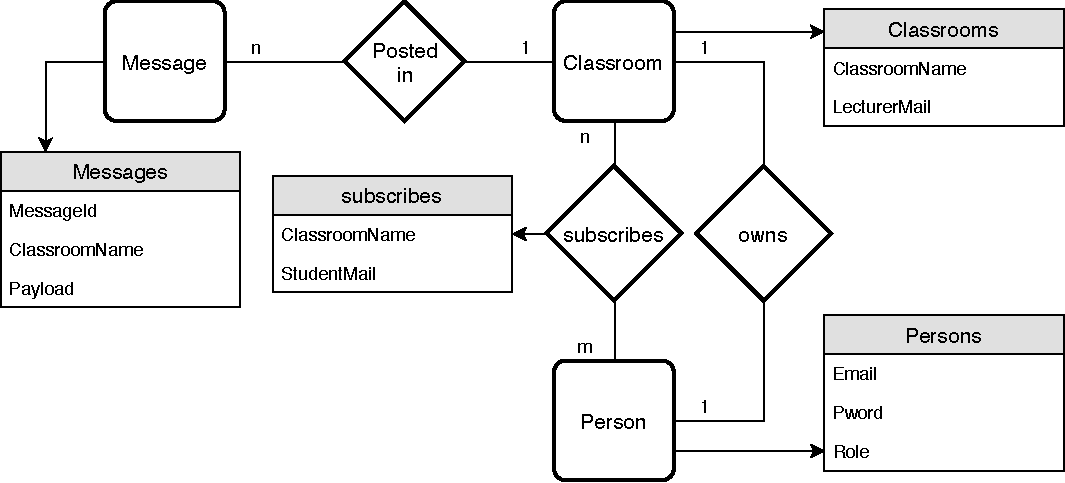
\includegraphics[scale=0.8]{Resources/EntityRelationship}
	\caption{Entity-Relationship Modell der Datenbank}
	\label{pic:entityRelationship}
	\end{center}
\end{figure}
\newpage
\subsection{REST-API}
Als Schnittstelle zwischen Backend und App dient eine RESTful-API.
Verschiedene Daten sind über Endpoints (siehe Tabelle \ref{table:endpoints}) abrufbar, welche jeweils mit einer eindeutigen URI adressiert sind. 
Jeder dieser Endpoints ist einem bestimmtem Anwendungsfall zugeordnet, zum Abrufen der Daten muss der Http-Client einen POST-Request senden, der die geforderten Argumente im JSON-Format enthält.
Für Besseres Verständnis ist in Abbildung \ref{pic:rest} ein Beispiel angegeben: für den Login sendet die App einen POST-Request, welcher die Anmeldedaten enthält; der Server antwortet dann mit der Rolle des zugehörigen Benutzers.
Der Vorteil dieser Art von Schnittstelle liegt darin, dass das Backend \textit{stateless} -- also ohne Wissen über den Status des Clients -- implementiert werden kann.
Jedoch müssen bei der Abfrage jeder Ressource die Anmeldedaten des Benutzers gesendet werden.
Darüber hinaus gestaltet sich so die Umsetzung der Serverstruktur als einfach, da sie so ohne Nebeneffekt erweiterbar ist.
Der Hauptgrund für die Wahl einer RESTful-Schnittstelle ist jedoch, dass sie unabhänig vom System implementiert werden kann. 
Es wäre also beispielsweise ohne weiteres möglich neben der App auch eine Webanwendung zu erstellen, welche sich ebenfalls mit dem Backend verbindet.

\begin{figure}[H]
	\begin{center}
	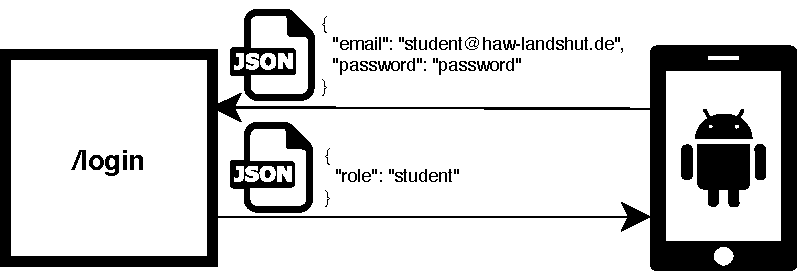
\includegraphics[scale=0.8]{Resources/RESTAPI}
	\caption{Beispiel für Kommunikation mit der REST-API}
	\label{pic:rest}
	\end{center}
\end{figure}

\begin{table}[H]
\begin{tabular}{l|l|l}
\textbf{Endpoint URI} & \textbf{Argumente}  & \textbf{Rückgabewert}\\ \cline{1-3}
/classrooms/all & Student-Anmeldedaten & alle Kursräume und Status  \\ \cline{1-3}
/classrooms/subscribed & Student-Anmeldedaten & alle abonnierten Kursräume \\ \cline{1-3}
/classrooms/subscribe & Student-Anmeldedaten, Kursraumname & Erfolg \\ \cline{1-3}
/classrooms/unscribe & Student-Anmeldedaten, Kursraumname & Erfolg \\ \cline{1-3}
/classrooms/create & Dozent-Anmeldedaten, Kursraumname & Erfolg \\ \cline{1-3}
/classrooms/delete & Dozent-Anmeldedaten, Kursraumname & Erfolg \\ \cline{1-3}
/classrooms/owned & Dozent-Anmeldedaten & alle Dozenten-Kursraume\\ \cline{1-3}
/login & Anmeldedaten & Benutzerrolle \\ \cline{1-3}
/messages/student & Student-Anmeldedaten & abonnierte Nachrichten \\ \cline{1-3}
/messages/create & Dozent-Anmeldedaten, Kursraumname, Text &  Erfolg\\ \cline{1-3}
/messages/delete & Dozent-Anmeldedaten, id & Erfolg\\ \cline{1-3}
/messages/classroom & Anmeldedaten, Kursraumname & Kursraumnachrichten\\ \cline{1-3}
\end{tabular}
\caption{Liste aller Endpoints und deren Argumente beziehungsweise Rückgabewerte}
\label{table:endpoints}
\end{table}













